%%%%%%%%%%%%%%%%%%%%%%%%%%%%% Define Article %%%%%%%%%%%%%%%%%%%%%%%%%%%%%%%%%%
\documentclass[a4paper]{article}
%%%%%%%%%%%%%%%%%%%%%%%%%%%%%%%%%%%%%%%%%%%%%%%%%%%%%%%%%%%%%%%%%%%%%%%%%%%%%%%

%%%%%%%%%%%%%%%%%%%%%%%%%%%%% Using Packages %%%%%%%%%%%%%%%%%%%%%%%%%%%%%%%%%%
\usepackage{geometry}
\usepackage{graphicx}
\usepackage{amssymb}
\usepackage{amsmath}
\usepackage{amsthm}
\usepackage{booktabs}
\usepackage{lipsum}
\usepackage{graphicx}
\usepackage{color}
\usepackage{nth}
\usepackage{bm}
\usepackage{caption}
\usepackage{subcaption}
\usepackage{url}
\usepackage{hyperref}
\usepackage{array}
\usepackage{multirow}
\usepackage{parskip}
%%%%%%%%%%%%%%%%%%%%%%%%%% Page Setting %%%%%%%%%%%%%%%%%%%%%%%%%%%%%%%%%%%%%%%
\geometry{a4paper}

% sans-serif font
\renewcommand{\familydefault}{\sfdefault}

%%%%%%%%%%%%%%%%%%%%%%%%%% Define some useful colors %%%%%%%%%%%%%%%%%%%%%%%%%%
\definecolor{ocre}{RGB}{243,102,25}
\definecolor{mygray}{RGB}{243,243,244}
\definecolor{deepGreen}{RGB}{26,111,0}
\definecolor{shallowGreen}{RGB}{235,255,255}
\definecolor{deepBlue}{RGB}{61,124,222}
\definecolor{shallowBlue}{RGB}{235,249,255}
%%%%%%%%%%%%%%%%%%%%%%%%%%%%%%%%%%%%%%%%%%%%%%%%%%%%%%%%%%%%%%%%%%%%%%%%%%%%%%%

%%%%%%%%%%%%%%%%%%%%%%%%%% Macros %%%%%%%%%%%%%%%%%%%%%%%%%%%%%%%%%%%%%%%%%%%%%
\DeclareMathOperator{\Lagr}{\mathcal{L}}
%%%%%%%%%%%%%%%%%%%%%%%%%%%%%%%%%%%%%%%%%%%%%%%%%%%%%%%%%%%%%%%%%%%%%%%%%%%%%%%


\begin{document}
% custom title page
\begin{titlepage}
  \begin{center}

    \vspace*{1cm}

    \textbf{\LARGE
    % Training and Deploying Computer Vision Models for Indoor Localisation
    % Exploring Deep Learning for Indoor Localisation: A Study on Room-Level Accuracy
    Navigating Indoors with Computer Vision: Exploring Deep Learning Approaches
    for Room-Level Indoor Localisation
    % Deep Learning for Accurate Room-Level Indoor Localisation: Feasibility and Evaluation
    % Enhancing Indoor Spatial Awareness: Deep Learning Approaches for Room-Level
    % Indoor Localisation
    }

    \vspace{1.5cm}

    % author
    \begin{minipage}[t]{5cm}
      \centering
      \textbf{Mika Senghaas} (Author) \\
      IT University of Copenhagen \\
      \textit{jsen@itu.dk}
    \end{minipage}
    \hspace{1cm}
    \begin{minipage}[t]{5cm}
      \centering
      \textbf{Stella Grasshof} (Supervisor) \\
      IT University of Copenhagen \\
      \textit{stgr@itu.dk}
    \end{minipage}

    \vfill

    % degree
    A Thesis presented for the Degree of \\
    \textbf{Bachelor of Science in Data Science}

    \vspace{0.8cm}

    
\includegraphics[width=0.4\textwidth]{figures/itu.jpg}

    \vspace{0.8cm}

    \textbf{IT University of Copenhagen}\\
    Computer Science Department\\
    \vspace{.5cm}
    May, 15th 2023

  \end{center}
\end{titlepage}

\newpage

% table of contents, list of tables, list of figures
\tableofcontents
% \listoftables
% \listoffigures
\newpage

\begin{abstract} % (fold)

Despite decades of research efforts, indoor localisation remains a challenging
task. One reason for this is that current approaches are typically designed with
the requirement of centimetre-accuracy in mind. Motivated by the success of deep
learning in numerous computer vision tasks, this study investigates the
applicability of deep learning techniques to the task of indoor localisation
when relaxing the constraint of centimetre-accuracy and viewing localisation as
a classification task. Various deep learning architectures are trained and
evaluated on a novel video dataset for indoor localisation. The study shows that
both single-frame and video models are capable of providing reasonably accurate
localisation results, even when trained on a small dataset, but are limited to
differentiate between areas of similar appearance. Nevertheless, the results are
promising, and give hope for the method to be applicable in real-world
scenarios.

\end{abstract}

\section{Introduction}
\label{sec:introduction}

% outdoor localisation as solved problem 
With the introduction of the satellite-based Global Positioning Systems
(GPS), localisation in outdoor spaces has become more efficient and accurate
than ever before. Gradual commercialisation led to the technology rapidly
transforming industries and personal navigation. Today, outdoor localisation is
widely considered a \textit{solved problem}.

% gps struggles in indoor spaces
The same cannot be said for indoor localisation. Because the transmitted radio
signals sent out by the satellites in GPS systems are not strong enough to
penetrate through walls and struggle with reflections from large buildings, the
technology yields inaccurate results at best, and often becomes dysfunctional in
indoor spaces~\cite{survey1, survey2}.

% indoor localisation techniques (broad overview)
With the ongoing urbanisation and the emergence of autonomous robots and
vehicles, the need for indoor localisation technologies is growing. Over the
past decades, a wide variety of solutions have been proposed:
Infrastructure-based systems use radio signals, transmitted by beacons, like
Bluetooth~\cite{bluetooth1, bluetooth2}, Ultra-Wideband (UWB)~\cite{uwb1, uwb2}
or Wi-Fi~\cite{survey1, survey2, wireless-positioning}, to localise an agent in
a known environment. Infrastructure-less systems, like simultaneous localisation
and mapping (SLAM) algorithms, rely solely on sensors, like
cameras~\cite{mono-slam, ptam, orb-slam} or distance-measuring
lasers~\cite{lidar-slam} to localise an agent in an unknown environment.

% short-comings of existing approaches
While these approaches have produced remarkable results, being capable of
localising an agent with centimetre accuracy, they are limited for various
reasons: Infrastructure-based systems require an initial setup and maintenance
of the installed hardware, which makes them costly, time-intensive and difficult
to implement in large environments. Infrastructure-less systems, on the other
hand, require complex processing of the sensory information and need to be
fine-tuned by experts for each indoor space, to achieve outstanding results.
These limitations have prevented existing solutions from being more wide-spread
adoption in use-cases like personal navigation in indoor spaces.

% short-comings of existing approaches
Previous approaches were designed under the assumption that centimetre-accuracy
is categorically required. However, not all use-cases require
centimetre-accuracy, and in many cases, the cost of the implementation of an
accurate system is not justified. For example, in a museum or shopping floor, it
might be sufficient to know in which area a visitor is. In these cases, the
constraint of centimetre-accuracy can be relaxed, in favour of a simpler and
more versatile solution.

% offline solution
% run in real time on mobile device
% during inference no setup required in the environment
% useable in an indoor space by a human or autonomous agent with camera

% success of deep learning in computer vision
Deep learning, which is part of a broader family of machine learning methods,
has recently gained a lot of attention in the field of computer vision and
proven to be a powerful tool for solving a wide variety of tasks. Amongst the
most common tasks in computer vision are image and video classification, where
the goal is to predict a label from a set of pre-defined labels for a given
image or video. It is natural to ask (a) whether the task of indoor
localisation can be phrased as a coarse-grained classification task, where
labels correspond to areas in an indoor space, and (b) whether deep learning
techniques can be used to produce accurate localisation results in this setting.

% deep learning for indoor localisation
Therefore, this study investigates the applicability of modern deep learning
techniques to the task of indoor localisation when viewing localisation as a
classification task. The study presents the rigorous evaluation of several deep
learning models on a challengingly small video dataset for mapping out a novel
indoor space in this setting.

% contributions
The main contributions are:

\begin{enumerate} 

  \item A novel, small single-frame and video classification dataset for indoor
    localisation based on ~40 minutes of video footage in 20 different rooms.

  \item A rigorous evaluation of several modern deep learning architectures on
    the task of indoor localisation, when viewed as a classification task.

  \item A discussion of the results and an outlook on the applicability of a
    pure deep learning pipeline to the task of indoor localisation.

\end{enumerate}

% section introduction (end)

% \section{Motivation} % (fold)
% \label{motivation}
% 
% This study is motivated by (a) the apparent lack of single, wide-spread indoor
% localisation systems and (b) the success of deep learning in computer vision in
% numerous computer vision tasks. This section gives a brief overview of the
% current state of indoor localisation, reviews the success of deep learning in
% many computer vision to, finally, motivate the study of deep learning for indoor
% localisation in a classification setting.
% 
% \subsection{Existing Solutions for Indoor Localisation}
% 
% Indoor localisation is at the core of numerous applications, such as autonomous
% robots and vehicles, augmented reality, or indoor navigation systems. With the
% above technologies becoming increasingly capable and affordable, the need for
% indoor localisation technologies grows. This section gives a
% comprehensive overview of previously studied approaches to indoor localisation.
% The approaches are broadly categorised into those that rely on infrastructure
% being present (infrastructure-based) in the indoor space and those that do not
% (infrastructure-less).
% 
% \subsubsection{Infrastructure-based Indoor Localisation Systems} % (fold)
% 
% GPS fails in indoor spaces because the signal transmitting satellites are too
% far away from the receiver. Over the large distance, the signal is not strong
% enough to penetrate through walls and there is a high chance for reflections
% that distort the signal. While this makes GPS a poor choice for indoor
% localisation, its success in outdoor spaces has inspired similar systems in
% indoor spaces.
% 
% Infrastructure-based indoor localisation systems replace the satellites with
% close-proximity beacons, such as Bluetooth~\cite{bluetooth1, bluetooth2},
% Ultra-Wideband (UWB)~\cite{uwb1, uwb2} or Wi-Fi~\cite{survey1, survey2}.
% Independently of the choice of the radio signal, three main approaches can be
% distinguished: 
% 
% \begin{enumerate}
%   \item \textbf{Angle of Arrival (AOA).} In AOA approaches, beacons are
%     measuring the distance and angle between the beacon and the agent. The
%     intersection between the line of sight of at least three beacons yields the
%     position of the agent.
% 
%   \item \textbf{Time of Arrival (TOA).} TOA approaches (such as GPS) use the
%     received signal strength (RSS) to estimate the distance between an agent and
%     the AP. In a process called multilateration, an agent's
%     position can be determined as the intersection of four spheres with known
%     radius (distance estimates) and centres (known position).
% 
%   \item \textbf{Received Signal Strength Fingerprinting (RSSI-FP).} RSSI-FP
%     approaches~\cite{survey1, survey2} involve two separate phases: First, an
%     offline phase, maps the indoor environment by associating a set of chosen
%     reference points (RPs) with a vector of received signal strength indicator
%     (RSSI) values of the APs. In the online phase, the agent's position is then
%     determined by dynamically comparing the agent's RSSI vector against the RSSI
%     vectors of the RPs stored in the database, and determines the agent's
%     position as the position of the RP with the most similar RSSI vector
%     according to some similarity metric.
% 
% \end{enumerate}
% 
% AOA and TOA methods require precise knowledge of the positions of the APs,
% which is often not available. RSSI-FP approaches do not require such knowledge,
% but are sensitive to changes in the environment and require a time-intensive
% offline mapping phase. Furthermore, all of the above approach rely on measured
% radio signal strength, which is known to be prone to errors, especially in
% indoor spaces that are dense, cluttered, and dynamic~\cite{survey1}. Moreover,
% they assume massive infrastructure deployments, which incur high setup and
% maintenance costs. 
% 
% In summary, infrastructure-based indoor localisation systems can provide
% accurate location estimates, but require a large infrastructure deployment,
% which is not feasible in many real-world scenarios.
% 
% \subsubsection{Infrastructure-less Indoor Localisation Systems} % (fold)
% 
% The inherent limitations of infrastructure-based indoor localisation systems
% have motivated the development of infrastructure-less indoor localisation
% systems. Such systems do not require any setup in the location, but rely on
% sensory information from the agent itself.
% 
% % slam
% Amongst the most promising approaches are SLAM (Simultaneous Localisation and
% Mapping) algorithms. SLAM algorithms aim to localise an agent inside an
% unknown environment, while simultaneously building a consistent map of the
% environment. There exist a variety of different approaches to SLAM, depending
% on the type of sensors that are used. For example, Visual SLAM (V-SLAM)
% algorithms use camera input, and LidarSLAM algorithms use distance-measuring
% laser sensors. 
% 
% Most related to this study are monocular V-SLAM algorithms, because they use a
% single camera to estimate the position of the agent. The first monocular
% feature-based V-SLAM algorithms, MonoSLAM, was proposed in
% 2007~\cite{mono-slam}.  Since then, many adjustments and optimisation have been
% proposed to the algorithm to make it more robust and accurate. Typically, the
% adjustments replace or modify one of the components of the pipeline. For
% example, the ORB-SLAM~\cite{orb-slam} algorithm uses a bag-of-words approach for
% feature matching, and the PTAM~\cite{ptam} parallelises the computation for
% positioning and map creation, which was shown to improve the accuracy of the
% algorithm. 
% % In recent years, modifications are often based on deep learning techniques to
% % improve parts of traditional SLAM pipelines. For example, the
% % DeepVO~\cite{deep-vo} algorithm uses a convolutional neural network to
% % estimate the camera pose from a sequence of images. 
% 
% Overall, SLAM algorithms are promising for indoor localisation due to their
% precision and versatility. They do not require any infrastructure and can
% operate in unknown environments without prior knowledge of the environment. This
% makes them the method of choice for many autonomous robots, like vacuum robots,
% which automatically navigate in unknown, indoor environments. However, SLAM
% algorithms are computationally expensive and require a lot of memory. This makes
% them less suitable for mobile devices, which are often resource-constrained.
% Furthermore, to achieve outstanding results, the SLAM pipeline needs to be
% fine-tuned to the specific environment and use-case, which can only be done by
% experts. This makes SLAM algorithms less suitable for general-purpose indoor
% localisation.
% 
% \subsection{The Success of Deep Learning in Computer Vision} % (fold)
% 


\section{Background} % (fold)
\label{sec:background}

Phrasing the problem of indoor localisation as a classification problem and
solving it with a pure deep learning approach requires a brief introduction to
some of the fundamentals that underlie the methods used in this study. This
section, therefore, introduces the fundamental concepts of deep learning that
are relevant to this study.

\subsection{Fundamentals of Machine and Deep Learning}

Machine learning is a subfield of artificial intelligence (AI) that describes a
series of techniques and algorithms that allow computers to learn from data
without being explicitly programmed. One example of a machine learning task is
classification, which aims to assign a discrete label $\hat{y} \in \{y_1,
\ldots, y_n\}$ to an input $x$. The mapping from the input $x$ to the label
$\hat{y}$ is called a classifier, and often denoted as $\hat{f}(x) = \hat{y}$.
Typically such a classifier is trained on a large set of labelled data, called
the training set, which consists of true instances $x_i$ and their labels $y_i$.
Using numeric optimisation algorithms, like gradient-descent, the classifier
iteratively improves its approximation $\hat{f}$ of the true mapping $f(x) = y$
by minimising a loss function $\mathcal{L}(\hat{f}(x), y)$ that quantifies the
error of the machine learning model.

Deep learning is a subfield of machine learning, and describes a specific class
of machine learning algorithms that are based on the theory of artificial neural
networks (ANNs). ANNs are inspired and loosely related to the structure and
functioning of the neurons in the human brain. They are structured in a series
of fully-connected layers, where each layer consists of a number of nodes.
Figure~\ref{fig:ann} shows an ANN with an input layer with three nodes, three
hidden layers with seven nodes each and an output layer with three nodes.
Information flows from the input layer through the hidden layers to the output
layer. The information happens through sequential linear transformations of the
input data, which are performed by the nodes in the network. Specifically, each
node's output is a linear transformation of the outputs of all nodes in the
previous layer, 

\begin{equation}
  z_{i} = \sum_{j=1}^{n} w_{ij} x_j + b_i
  \label{eq:perceptron}
\end{equation}

where $x_j$ is the output of the $j$-th node in the previous layer, $w_{ij}$ is
the weight of the connection between the $j$-th node in the previous layer and
the $i$-th node in the current layer, $b_i$ is the bias of the $i$-th node in
the current layer, and $z_i$ is the output of the node.

Before the output $z_i$ is passed to the next layer, it is transformed by a
differentiable, non-linear activation function $\sigma$ to produce an activation
$a_i = \sigma(z_i)$. Once all activations in the $j$-th layer are computed, the
next layer can be computed by applying the same process to the activations of
the previous layer. This process, referred to as forward propagation, is
iteratively repeated until the activations in the output layer are computed,
which are the final outputs of the network.

Critically, the linear transformations performed by each node are parametrised
by weights, which are optimised during training. This allows ANNs to learn
complex non-linear mappings given enough samples of the input-output
relationship without explicitly programming the mapping. This makes ANNs a
powerful tool to solve a variety of complex machine learning tasks.

\begin{figure}
  \begin{center}
    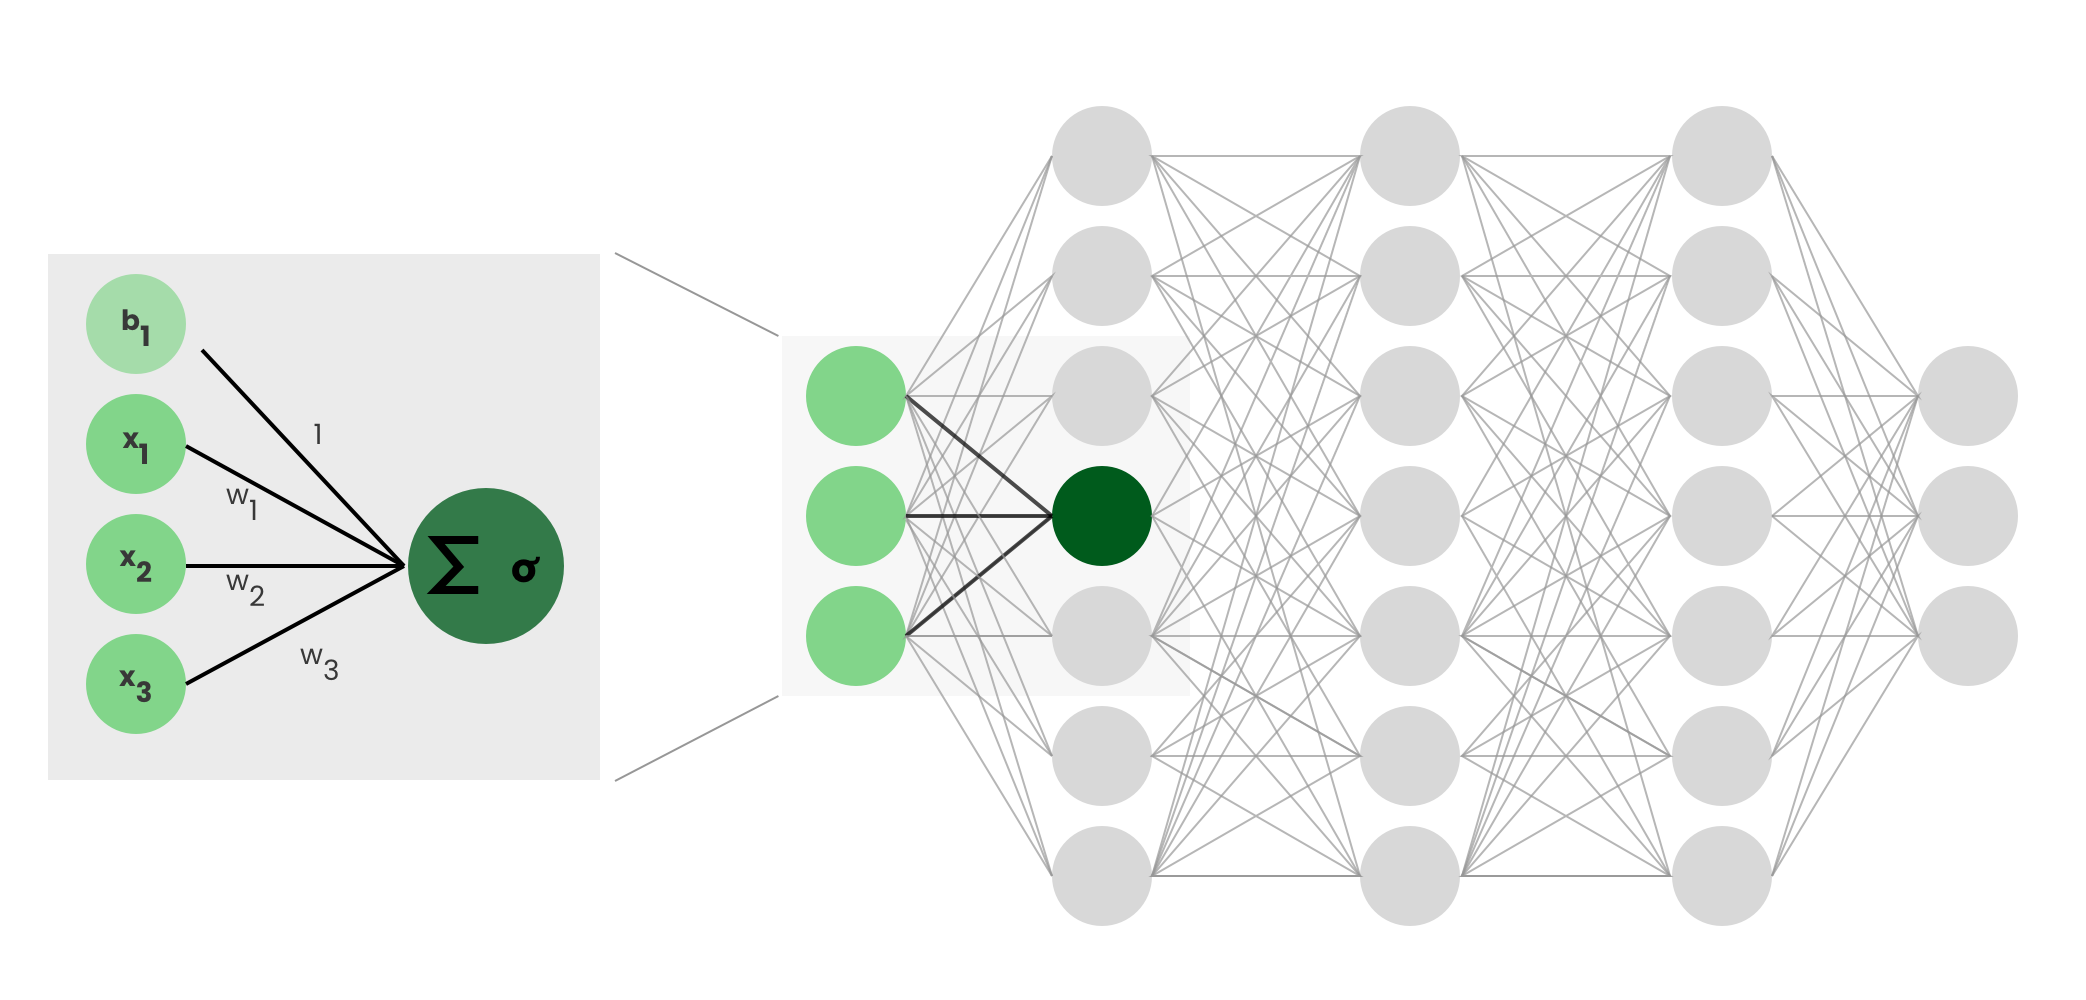
\includegraphics[width=\textwidth]{./figures/ann.png}
  \end{center}

  \caption{\textbf{Artificial Neural Network.} A schematic of the fundamental
    building blocks of an artificial neural network (ANN). The right figure
    shows the macro structure of an exemplary ANN with an input layer, three
    hidden layers, and an output layer. The left figure shows the micro
    structure of a single node in the network. The node performs a linear
    transformation of the inputs $x_i$ and the weights $w_i$ and adds a bias
    $b_i$. The output of the node is the result of a non-linear activation
    function $\sigma$ applied to the linear transformation.}
  \label{fig:ann}
\end{figure}

\subsection{Image Classification}
\label{sub:image-classification}

Image classification is one of the most fundamental and widely studied tasks in
computer vision and describes the process of assigning a label $y \in \{y_1,
\ldots, y_n\}$ to an image $x$ with dimensions $c \times h \times w$, where $c$
denotes the number of colour channels, $h$ denotes the height, and $w$ denotes
the width of the image.

Extracting information from images to assign a label is not straight-forward,
because of the high-dimensional and unstructured nature of images. These
characteristics make it challenging for traditional heuristic-based algorithms
to extract meaningful information, which has long limited the capabilities of
computer vision systems. However, with the advent of deep learning and the
introduction of a special type of neural network, called convolutional neural
network (CNN), this has changed.

CNNs are a type of neural network, which are inspired by the visual cortex,
which is responsible for processing visual information. Like the visual cortex,
CNNs are organised hierarchically and traditionally consist of convolutional,
pooling and fully-connected layers. Convolutional layers are the core of CNNs
and are responsible for extracting features from the input. Each convolutional
layer consists of a set of $c_o$ filters $k_1, \ldots, k_{c_o}$, where
each $k_i$ is a three-dimensional matrix of weights with dimensions $c_i \times
h_k \times w_k$, where $c_i$ is the number of channels in the input, and $h_k$
and $w_k$ are the height and width of the filter. Given an input $x$ with
dimensions $c_i \times h_i \times w_i$, a single convolutional filter $k$
produces a feature map $z$ by sliding the filter across the input and computing
the convolution at each position ${i,j}$, as 

\[
  z_{i,j} = \sum_{c=1}^{c_i} \sum_{m=1}^{h_k} \sum_{n=1}^{w_k} 
  k_{c,m,n} x_{c,i+m,j+n}
\]

Each convolutional filter produces a two-dimensional feature-map $z$, which are
stacked along the channel dimension to produce a three-dimensional output of
size $c_o \times h_o \times w_o$. After applying a non-linear activation, the
output of the convolutional layer becomes the input of a deeper layer.
Typically, the output of a convolutional layer is passed on to a pooling layer,
which is related to the convolutional layer, because it also contains a set of
sliding filters. However, instead of computing a convolution, the filters in the
pooling layer compute a statistic, such as the maximum (Max Pooling) or average
(Average Pooling), of the values in the kernel. 

% why cnns work
CNNs have been found to work specifically well for data with a spatial structure
such as images. This is because the convolution operation models the inherent
structure of images: While a stand-alone pixel is not informative, the value of
a pixel in the context of its neighbouring pixels is. This characteristic is
naturally captured by the convolution operation. Furthermore, in sliding filters
across the input, they can capture the same feature independently of its
location in the image.

% why cnns work
The first CNN-based architectures date back to the 1960s and have shown
successes in simple image classification tasks~\cite{lenet}. However, it was not
until 2012, when the CNN-based architecture AlexNet~\cite{alexnet} won the
ImageNet Large Scale Visual Recognition Challenge (ILSVRC)~\cite{imagenet}, that
CNNs arrived in the mainstream of computer vision. Since then CNNs have been
proposed in various different forms, mostly differing in the network's structure
and depth and the width and resolution of the filters. To this day, CNNs still
rank amongst the top performing methods in image classification benchmarks.

\begin{figure}
  \centering
  \begin{subfigure}[b]{0.49\textwidth}
    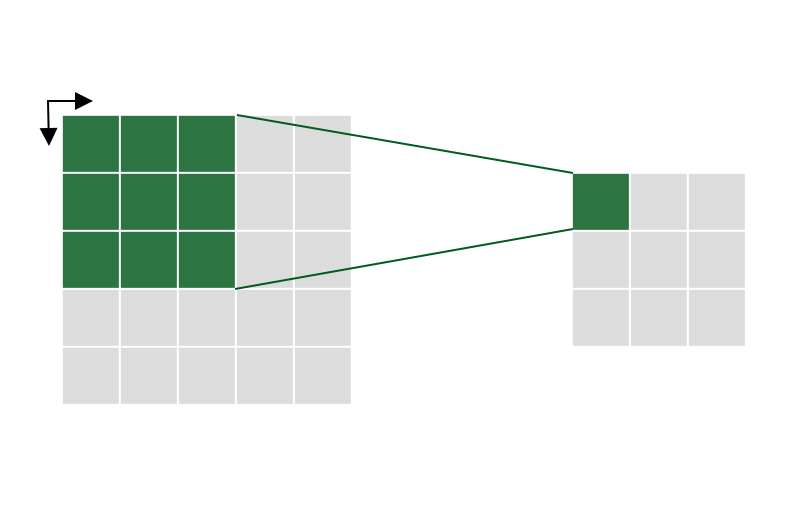
\includegraphics[width=\textwidth]{./figures/2d-conv.png}
    \caption{2d Convolution}
  \end{subfigure}
  \hfill
  \begin{subfigure}[b]{0.49\textwidth}
    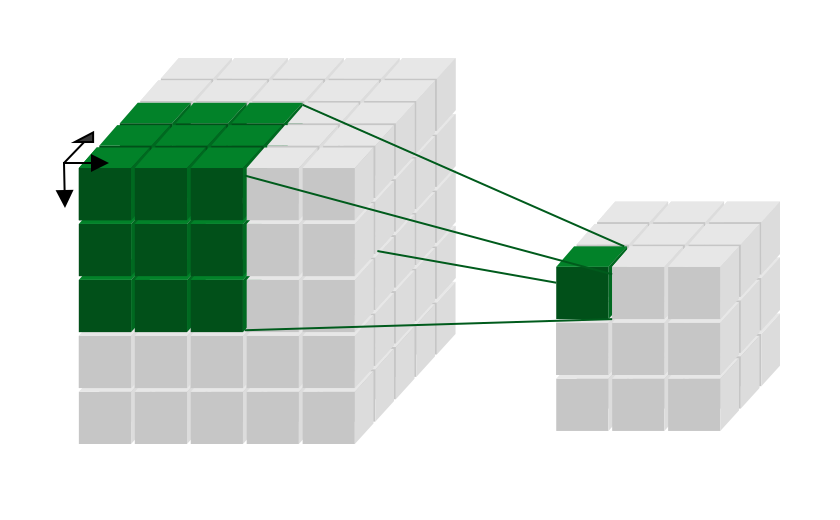
\includegraphics[width=\textwidth]{./figures/3d-conv.png}
    \caption{3D Convolution}
  \end{subfigure}
  \caption{
  \textbf{2D and 3D Convolution.} A simplified illustration striding of 2D and
  3D convolutional filters across an input. For visualisation purposes, a single
  channel is shown. A 2D convolutional filter (a) slides across the spatial
  dimension (height and width) of an input. A 3D convolutional filter (b) slides
across the spatio-temporal dimension (height, width, and time) of an input.}
  \label{fig:conv}
\end{figure}

\subsection{Video Classification}
\label{sub:video-classification}

Video classification can be seen as a generalisation of image classification:
Instead of assigning a label to a single image, video classification assigns a
label $y$ or a sequence of labels $y_1, \ldots, y_t$ to a video sequence $x =
(x_1, \ldots, x_T)$, where $x_t$ is a frame of the video.

The difference is subtle, yet important, because it introduces a temporal
dimension to the task. It is generally assumed that the temporal dimension
is critical for video classification, because it provides additional
information about the video. For example, it might be difficult to determine
whether a person is running or walking from a single frame, but trivial given
the motion captured by a sequence of frames.

Motivated by the need for a powerful model to capture the semantic content of
video data and the success of CNNs in image classification, researchers have
started to apply CNNs to video classification~\cite{videocnn, i3d, c3d, x3d,
slowfast}, where the networks have access to the complex spatio-temporal
evolution of the video. Over the course of the last decade, various approaches
based on CNNs have been proposed that exhibit different connectivity patterns
for modelling the temporal dimension of the video~\cite{videocnn}.

% naive solution: single frame with averaging
A naive solution, which ignores the temporal dimension entirely, is to predict a
label for each frame and then average the predictions. These single-frame models
are not capable of directly modelling the temporal dimension of the video, but
have been shown to perform surprisingly well~\cite{videocnn}. Different methods
for aggregation have been proposed, such as averaging~\cite{videocnn}, majority
votes, or using a neural architectures, such as recurrent neural networks (RNNs)
to learn the importance of each frame~\cite{lrcn} for the final
prediction.

% model temporal dimension directly through 3d convolutions
CNN-based architectures that model the temporal dimension directly usually
leverage 3D convolutions~\cite{c3d, i3d}. 3D convolutions are a natural
extension of 2D convolutions, as defined in
Section~\ref{sub:image-classification}. Instead of sliding a convolutional
filter across the spatial dimension of the input (Figure~\ref{fig:conv}a), a
3d-convolutional filter slides across the spatio-temporal dimension of the input
(Figure~\ref{fig:conv}b), which produces feature maps in spatio-temporal space
that are learned jointly. The 3D convolutional filter is defined as follows:

% TODO: mathematical operation of 3d-convolution
% \[
%   z_{c,i,j,k} = \sum_{m=1}^{M} \sum_{n=1}^{N} \sum_{l=1}^{L} k_{c,m,n,l} x_{c,i+m,j+n,k+l}
% \]

3D convolutions have been used in many different variants. Architectures range
from pure 3D convolution networks~\cite{i3d, c3d} to hybrid architectures that
combine 2D and 3D convolutions~\cite{x3d, slowfast}. Overall, the literature on
video classification is vast and complex. Despite the introduction of
large-scale datasets for video classification~\cite{kinetics},
the research field has not yet converged to a consensus about the best approach
for video classification.

\section{Methodology} % (fold)
\label{sec:methodology}

Because of this lack of consensus in the literature, this study aims to
understand how different CNN-based architectures perform when faced with the
task of assigning labels to a continuous stream of frames, a video, in an indoor
space. To this end, the study considers a wide-variety of different models that
are detailed in Section~\ref{sub:models}.

One major distinction between the different models, is whether or not they
operate on a single-frame or a sequence of frames. Because this distinction
impacts all steps of the study, from data processing to model evaluation, the
following two different problem settings are distinguished throughout the entire
study:

\begin{enumerate}

\item \textbf{Single-frame classification}: Given a continuous stream of frames,
  the task is to classify each frame individually.

\item \textbf{Video classification}: Given a continuous stream of frames, the
  task is to classify fixed-sized clips of the video.

\end{enumerate}

\subsection{Raw Data} % (fold)
\label{sub:raw-data}

Framing the problem of indoor localisation as a classification task requires a
labelled data set, which consists of sequentially-arranged pairs of inputs and
outputs, that map visual information to location labels. 

% videos
The raw data was collected from a single camera of a mobile device at a frame
rate of 30 FPS in high resolution ($2426\times 1125$). The mobile device was
hand-held by a human agent while walking around the main building of the
Southern Campus of the Copenhagen University (Danish: K\o{}benhavns Universitet,
KU) in Copenhagen S, Denmark. The large multi-storey building consists of a
total of six floors. The location was deemed compatible with this study, as it
showcases distinctive learnable indoor features (e.g. coloured walls,
architectural unique structures, etc.), but also challenges the model, for
example, due to areas that visually similar to each other (like libraries and
corridors). For the scope of this project, the data collection was limited to
the first two floors. This process yielded a set of videos $V = \{v_1, ...,
v_n\}$, where each video $v_i$ is a sequence of $k$ frames $f_1, ..., f_k$. Each
frame $f_i$ is a RGB image with dimensions $3 \times 2426 \times 1125$.

% labels
Each video $v_i$ is associated with a set of location labels $L = \{l_1, ...,
l_n\}$, where each location label $l_i$ identifies the location of the agent at
a specific time in the video. For the scope of this project 20 different
location labels were considered, which are identified by a descriptive name and
integer. Figure~\ref{fig:map} shows the floor plan of the first two floors of
the building, where each location class is mapped to a coloured region. The
location labels were assigned in close correspondence to the original floor
plan. This, however, led to some classes being a lot larger than others, which
is likely to result in a class imbalance. Annotation was performed manually by a
single human agent. Because changes in the location labels only occur at the
transition of rooms, the annotation process was simplified by annotating the
starting and ending time stamps of a location label, which were later
pre-processed to frame-by-frame annotations. 

% statistics of the data
A total of $n=53$ videos of varying length were recorded, with an average
duration of $\sim 57$s, amounting to a total number of $\sim 50$ minutes of
footage, or an equivalent of $\sim 90K$ frames. Out of the total 53 videos
that were recorded, 37 were used for training and 16 were used for testing.
Importantly, the videos in the training split were recorded in a single
session, while the videos in the test split were recorded on four separated
days, in a span of two to four weeks after the training data had been
recorded. This was done to ensure that the models were tested against unseen
data, to more accurately assess their generalisation capabilities. Indeed, the 
test data was recorded in different weather conditions, at different times of
the day, with different lighting conditions and, by pure chance, one of the
areas was repainted during the time between the recording of the training and
test data. With all these changes in mind, the test data is expected to be
as different from the training data, as it would be in a real-world scenario.

% figure
\begin{figure}
\centering

\begin{subfigure}[b]{.7\linewidth}
  \centering
  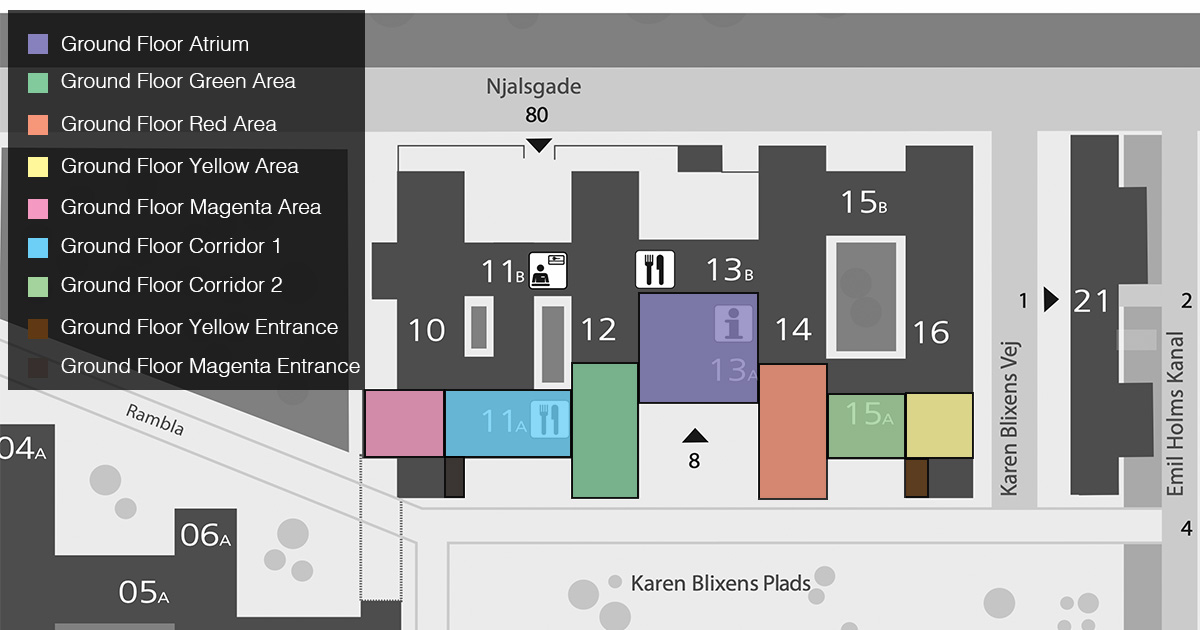
\includegraphics[width=\linewidth]{figures/map-ground-floor.jpg}
  \caption{Ground Floor}
  \label{fig:map-ground-floor}
\end{subfigure}

\hfill

\begin{subfigure}[b]{0.7\linewidth}
  \centering
  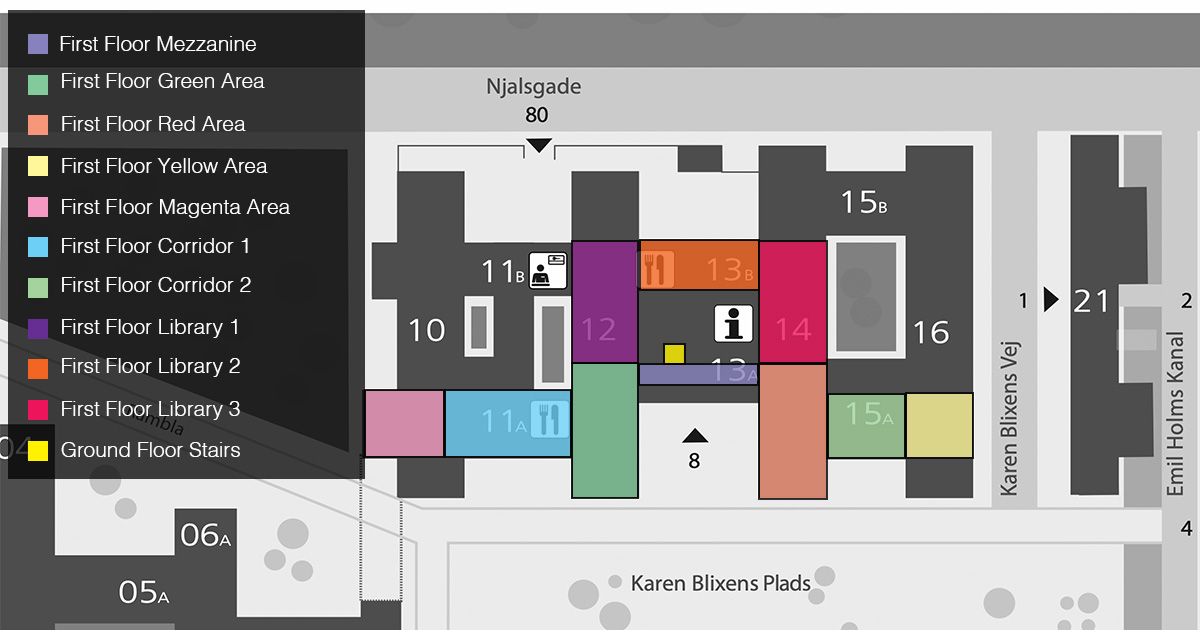
\includegraphics[width=\linewidth]{figures/map-first-floor.jpg}
  \caption{First Floor}
  \label{fig:map-first-floor}
\end{subfigure}

\caption{
  \textbf{Floor Plan of the Southern Campus of the Copenhagen with Location
  Labels.} The coloured regions represent the $|L|=20$ location labels as
  distributed over the two floors in the indoor space. It is apparent that
  a) the floor plan is similar across floors and b) that locations
  significantly differ in size.
}
\label{fig:map}
\end{figure}


% TODO: figure about the time of data collection (side-by-side, one where hue
%       denotes the split and the other where hue denotes the clips per day)

% subsection data-collection (end)

\subsection{Processed Data} % (fold)
\label{sub:processed-data}

\subsubsection{Single-Frame Dataset} % (fold)

% extraction of frames in training and testing
Single-frame classification models expect a single frame $f_i$ from a video
$v_i$ as input. Technically, all frames in a video $v_i$ could be used as input,
but because of the strong local correlation between adjacent frames, it was
hypothesised that models would overfit to the training data. For this reason,
and in an attempt to assimilate the single-frame and video datasets, frames from
a video $v_i$ were sampled at a sampling rate fixed $r_f$. The sampling rate is
not tied to the architecture of single-frame models and was therefore chosen
globally to be $r_f=5$ for the training split. This means that only every 5th
frame from the videos in the raw data split were used for training. A sampling
rate was not adopted for the testing split, in order to test the model on the
full set of frames.

% matching location
Matching the location labels to each of the extracted frames was
straight-forward. For each frame $f_i$ in a video $v_i$, the location label
$l_i$ was found as the label currently active at the time of the frame. This was
done by finding the location label $l_i$ that satisfied condition $t_{l_i} \leq
t_{f_i} \leq t_{l_{i+1}}$, where $t_{l_i}$ and $t_{f_i}$ are the time stamps of
the location label $l_i$ and frame $f_i$, respectively. This process yielded a
set of single-frame samples $D_F = \{(f_1, l_1), ..., (f_{n_f}, l_{n_f})\}$ with
$n_f=\sim 12K$ for the training split and $n_f=20K$ for the testing split.

\begin{figure}
\centering
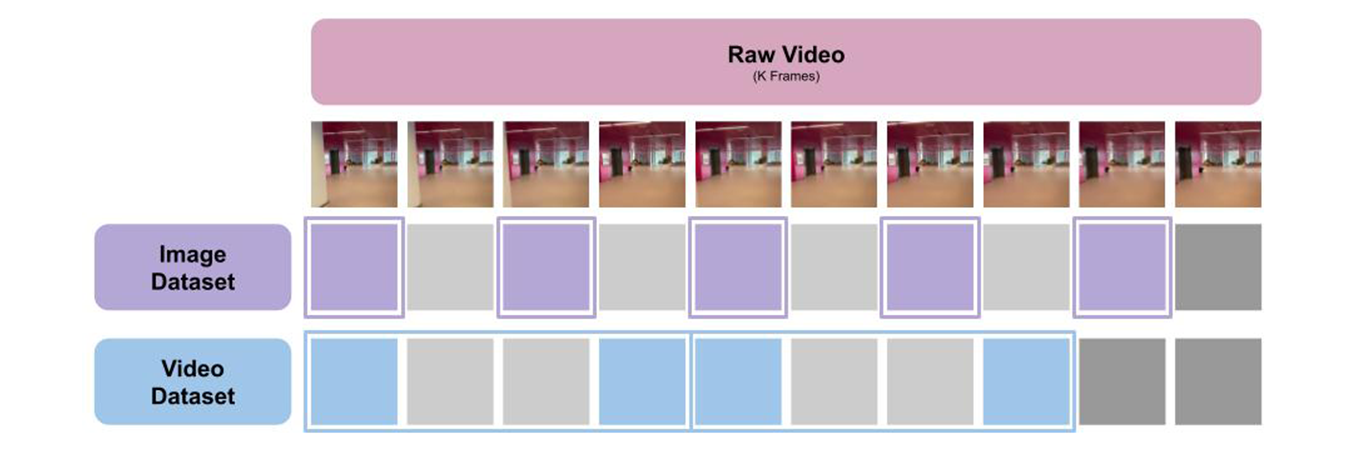
\includegraphics[width=0.95\textwidth]{figures/data-extraction.png}
\caption{
  \textbf{Data Extraction.} A raw video with $k=10$ frames is processed into
  $k_f=5$ frames for the single-frame dataset and $k_v=2$ clips for the
  video dataset. Samples for each dataset type are indicated by a
  surrounding box. Frames are sampled at a rate of $r_f=2$ for the
  single-frame dataset and $r_v=3$ for the video dataset. A clip contains
  $s_v=2$ frames. Frames are colour-coded in correspondence to the dataset
  they belong to (single-frame dataset in purple and video dataset in blue),
  if they are sampled to the respective dataset. Discarded frames are
  coloured in grey (light-grey for within video frames, dark-grey for
  trailing frames).}
\label{fig:data-extraction}
\end{figure}


\subsubsection{Video Dataset} % (fold)

A video classification models expects a single clip $c_i$ as input, which is a
fixed-sized sequence of $s_v$ frames sampled from a video $v_i$ at a sampling
rate $r_v$. For this reason, the video classification dataset is constructed by
extracting clips from the videos in the raw data split. Clips are extracted in
uniformly spaced intervals. Within this study only non-overlapping clips were
considered, meaning that in a single clip $c_i$, the location label $l_i$ is the
same for all frames $f_i \in c_i$. This is a simplification of the problem, as
it is possible for a person to move from one location to another within a single
clip, but was found more compatible with existing video classification
architectures. In reality, the simplification is viable, because during the
relatively small clip duration of $\sim 2$s, transitions between locations only
occur in a small subset of clips.

Because clips do not overlap multiple location labels, each clip $c_i$ can be
associated with a single location label $l_i$. The location label $l_i$ is found
as the location label present during the entire time span of the clip. This
process yielded a set of clip-location samples $D_V = \{(c_1, l_1), ...,
(c_{n_v}, l_{n_v})\}$.

\subsubsection{Dataset Comparison} % (fold)

The extraction of clips and frames for video and single-frame classification
models, respectively, is illustrated in Figure~\ref{fig:data-extraction}. It
shows that, despite the common raw data source, the frames considered in the two
datasets may not be the same. This is because of different sampling rates and
because adjacent clips reset the sampling rate. 

Assuming a single video $v_i$ with $k$ frames, the number of frames $k_f$ that
can be sampled from $v_i$ at a sampling rate $r_f$ is $k_f = \lfloor k / r_f
\rfloor$. The number of clips $k_v$ that can be sampled from $v_i$ at a sampling
rate $r_v$ is $k_v = \left\lfloor \frac{k}{r_v \cdot s_v} \right\rfloor \cdot
s_v$. 

It becomes clear, that


\[
  \left\lfloor \frac{k}{r_v \cdot s_v} \right\rfloor \cdot s_v \approx
  \left\lfloor \frac{k}{r_f} \right\rfloor, \quad \text{if} \quad r_v = r_f.
\]

For this reason, the sampling rate $r_f$ for the single-frame dataset was chosen
to be an as close as possible to the sampling rates of video classifiers. As
multiple video classifiers considered in this study have different sampling
rates ranging from $2$ to $8$, the sampling rate $r_f$ was chosen to be $5$.

This choice does not ensure that the two datasets are identical, but it ensures
that the total number of frames in each dataset is similar, which means that
all models visit similarly many frames during training.

Furthermore, it was hypothesised, that due to the large number of total frames
and strong local correlation between adjacent frames, the two datasets are
sufficiently similar to allow for comparison between the two model types.

% TODO: add statistics about nf and nv (number of frames and clips in train
% and test)

% subsection data-preprocessing (end)

\subsection{Models} % (fold)
\label{sub:models}


Following the literature on single-frame and video classification tasks, a
subset of twelve different models were trained and evaluated in this work.
Following the distinction made in Section~\ref{sec:methodology}, the models are
split into two categories single-frame and video classification models. 

Table~\ref{tab:model-overview} gives a comprehensive overview of the models. The
table shows the release year, the sampling rate $r_f$ for single-frame
classification models and the sampling rate $r_v$ and clip size $s_v$ for video
classification models. The table also shows the input size, the number of
parameters and the number of floating point operations (FLOPs) for a single
forward pass. Finally, the table shows the top-1 accuracy on the ImageNet
dataset~\cite{imagenet} for single-frame classification models and the top-1
accuracy on the Kinetics dataset~\cite{kinetics} for video classification, as
benchmarks for the models' performance.

The following section describes briefly explains the main architectural change
that differentiates the models. For a more detailed description of the models,
the reader is referred to the original papers.

% mention pre-processing

\begin{table}
  \centering
  \caption{
    \textbf{Model Overview.} The table shows all models that were evaluated in
    this work. The models are split into two categories: single-frame models and
    video models. For each model, the table reports the release year (Release),
    the frame rate (Rate) of the training data, the number of frames per clip
    (F/C; \textit{only applicable to video classifiers}), the spatial resolution
    (Size) of the input images, the number of parameters in millions (Params),
    the number of floating point operations in billions (FLOPs) and the
    benchmark Top-1 accuracy (Acc\@1) on ImageNet~\cite{imagenet} for
    single-frame classification models and the top-1 accuracy on the
    Kinetics~\cite{kinetics} dataset for video classification models. The table
    is sorted by release date within each group.
  }
  \begin{tabular}{cllllllll}
    \toprule
    & \multirow{2}{*}{\textbf{Model}} 
    & \bfseries Release & \bfseries Rate & \bfseries F/C & \bfseries Size &
    \bfseries Params & \bfseries FLOPs & \bfseries Acc@1 \\
    & & (Y) & ($r_f$/$r_v$) & ($s_v$) & ($h$, $w$) & (M) & (G) & (\%) \\
    \midrule
  \multirow{8}{*}{\rotatebox[origin=c]{90}{Single-Frame}} 
  & AlexNet~\cite{alexnet} & 2012 & 5 & - & 224 & 61.1 & 0.71 & 56.52 \\
  % & GoogLeNet~\cite{googlenet} & 2014 & 30 & - & 256 & 6.6 & 1.5 & 69.78 \\
  & ResNet18~\cite{resnet} & 2015 & 5 & -  & 224 & 11.7 & 1.81 & 69.76 \\
  & ResNet50~\cite{resnet} & 2015 & 5 & -  & 224 & 25.6 & 4.09 & 76.13 \\
  & DenseNet 121~\cite{densenet} & 2016 & 5 & - & 224  & 7.0 & 2.88 & 74.43 \\
  & MobileNet V3~\cite{mobilenetv3} & 2019 & 5 & - & 224  & 3.5 & 0.32 & 71.88 \\
  & ViT-B-16~\cite{vit} & 2020 & 5 & - & 224  & 86.7 & 17.56 & 81.07 \\
  & EfficientNet V2 S~\cite{efficientnetv2} & 2021 & 5 & - & 224  & 21.5 & 8.37 & 84.23 \\
  & ConvNext Tiny~\cite{convnext} & 2022 & 5 & - & 224  & 28.2 & 4.46 & 82.52 \\
  \midrule
  \multirow{4}{*}{\rotatebox[origin=c]{90}{Video}}
  & R(2+1)D~\cite{r2plus1d} & 2018 & 4 & 16 & 182 & 28.11 & 76.45 & 76.01 \\
  & Slow R50~\cite{slowfast} & 2018 & 8 & 8 & 224 & 32.45 & 54.52 & 74.58 \\
  & SlowFast R50~\cite{slowfast} & 2018 & 8 & 8 & 224 & 34.57 & 65.71 & 76.94 \\
  & X3D S~\cite{x3d} & 2020 & 6 & 13 & 182 & 3.5 & 2.96 & 73.33 \\
  \bottomrule
  \end{tabular}
  \label{tab:model-overview}
\end{table}

\subsubsection{Single-Frame Classifiers} % (fold)

\textbf{Alexnet}~\cite{alexnet} is a convolutional neural network that was
introduced by Krizhevsky \textit{et al.} in 2012. It was the first deep neural network to
win the ImageNet Large Scale Visual Recognition Challenge~\cite{imagenet} and is
considered to be one of the first successful application of deep learning to
image classification. Architecturally, it consists of five convolutional layers
with occasional max-pooling layers in between, followed by three fully connected
layers, as illustrated in Figure~\ref{fig:alexnet}.

\begin{figure}
  \centering
  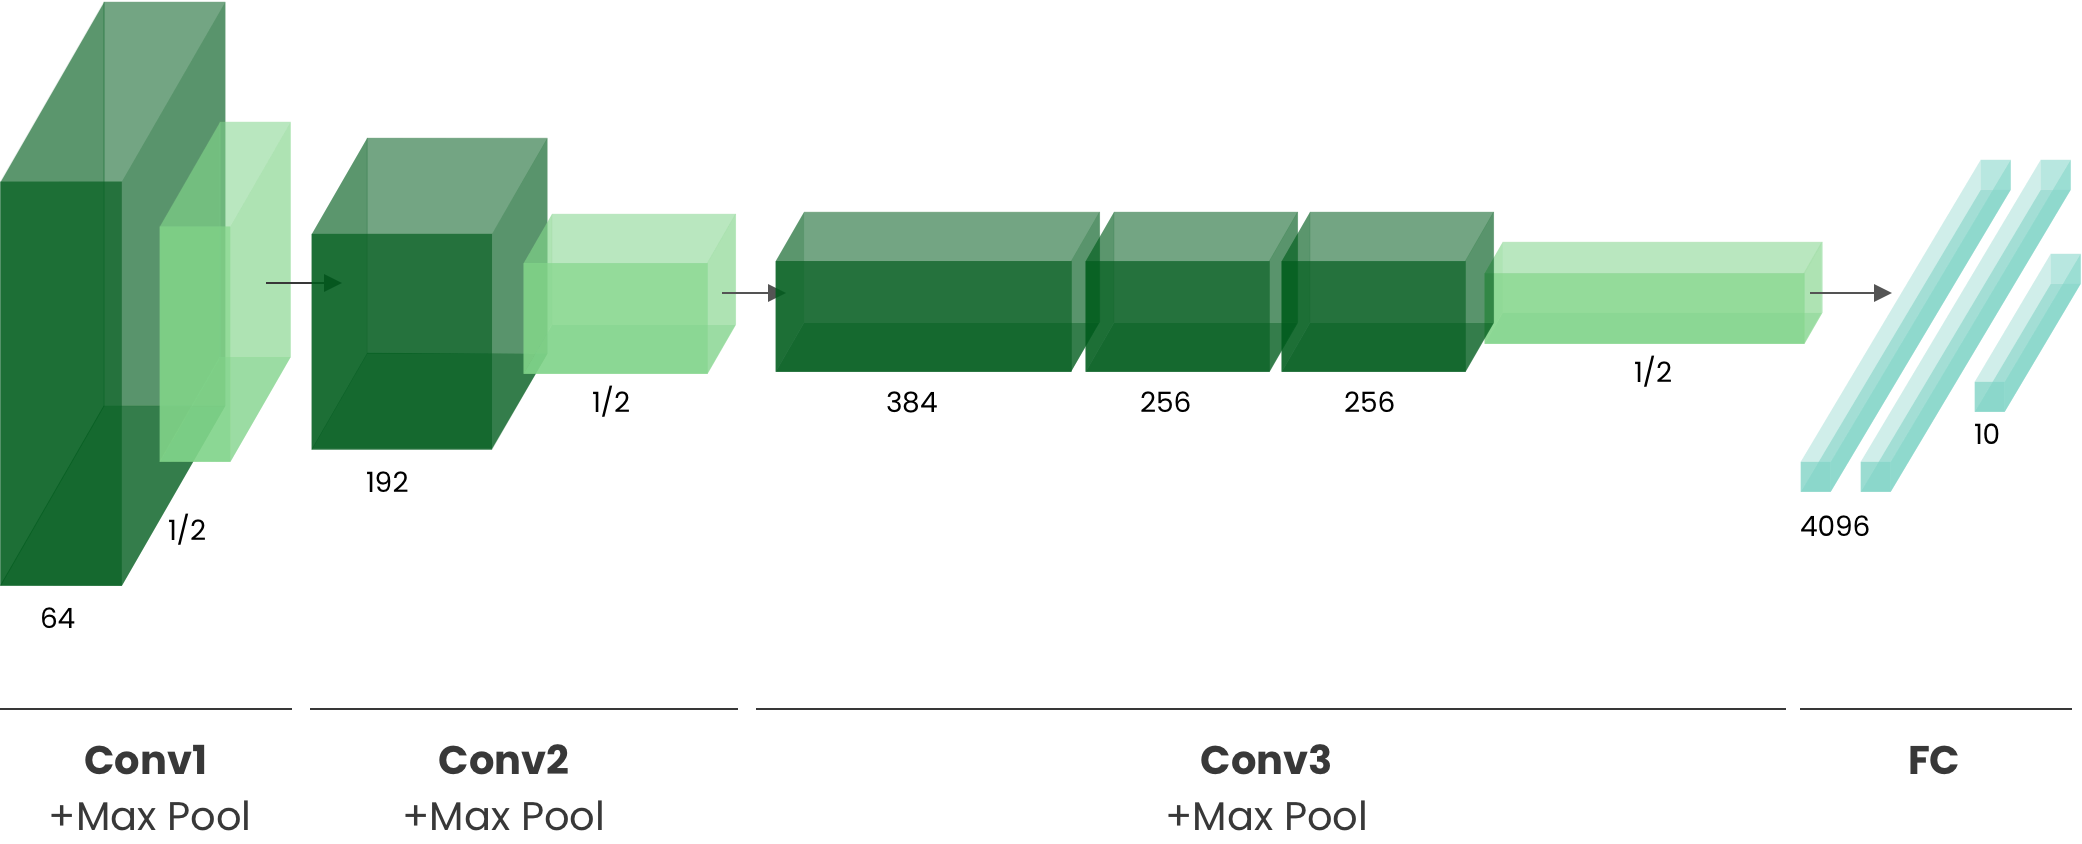
\includegraphics[width=\textwidth]{./figures/alexnet.png}
  \caption{\textbf{AlexNet Architecture.} An illustration of the architecture of
    AlexNet~\cite{alexnet}. Each box represents the output of a layer.
    Dark-green boxes are outputs of convolutional layers, light-green boxes are
    outputs of max-pooling layers and blue boxes are outputs of fully connected
    layers. The number of channels is denoted below each convolutional layer.
    Spatial downsampling is only performed by the first convolutional layer and
    all pooling layers. The downsampling factor is denoted below the pooling
    boxes.
  }
  \label{fig:alexnet}
\end{figure}

% \textbf{GoogLeNet} is a convolutional neural network that was introduced by
% Szegedy et al.~\cite{googlenet} in 2014. At its core, it is based on Inception
% modules, which allow the network to choose between multiple convolutional
% filter sizes in each block. Each inception module consists of 4 parallel
% convolutional layers, whose outputs are concatenated along the channel
% dimension. This advancement allowed the Google Team to significantly reduce
% the number of parameters in the network and win the ImageNet Large Scale
% Visual Recognition Challenge~\cite{imagenet} in 2014.

After the success of AlexNet, the speed of research in the field of deep neural
networks significantly picked up. Networks with increasing depth, such as
VGG~\cite{vgg}, were found to perform better, but led to new research problem:
As information about the input or gradient passes through many layers, it can
vanish during gradient-descent based learning, leading to a stagnation during
training. The phenomenon of "vanishing gradients" was visible in larger training
errors for deeper networks, and coined the "degradation" problem~\cite{resnet}. 

The \textbf{ResNet}~\cite{resnet} architecture is considered a cornerstone of
modern deep learning history as it introduced the concept of residual
connections. In a residual subnetwork of $L$ layers $H_l$, the output $x_l$ is
computed as the sum of the input to the subnetwork $x_{l-1}$ and the output of
the subnetwork $H_l(x_{l-1})$, i.e. $x_l=x_{l-1}+H_l(x_{l-1})$. The introduction
of this identify mapping to the output of the subnetwork was shown to facilitate
signal propagation in forward and backward paths, and, in connection with batch
normalisation~\cite{batchnorm}, allowed to train networks of unprecedented
length. The original paper introduced several architectures with different
depths, but in this work only ResNet18 and ResNet50, with 18 and 50 layers
respectively, are considered.

\begin{figure}
  \centering
  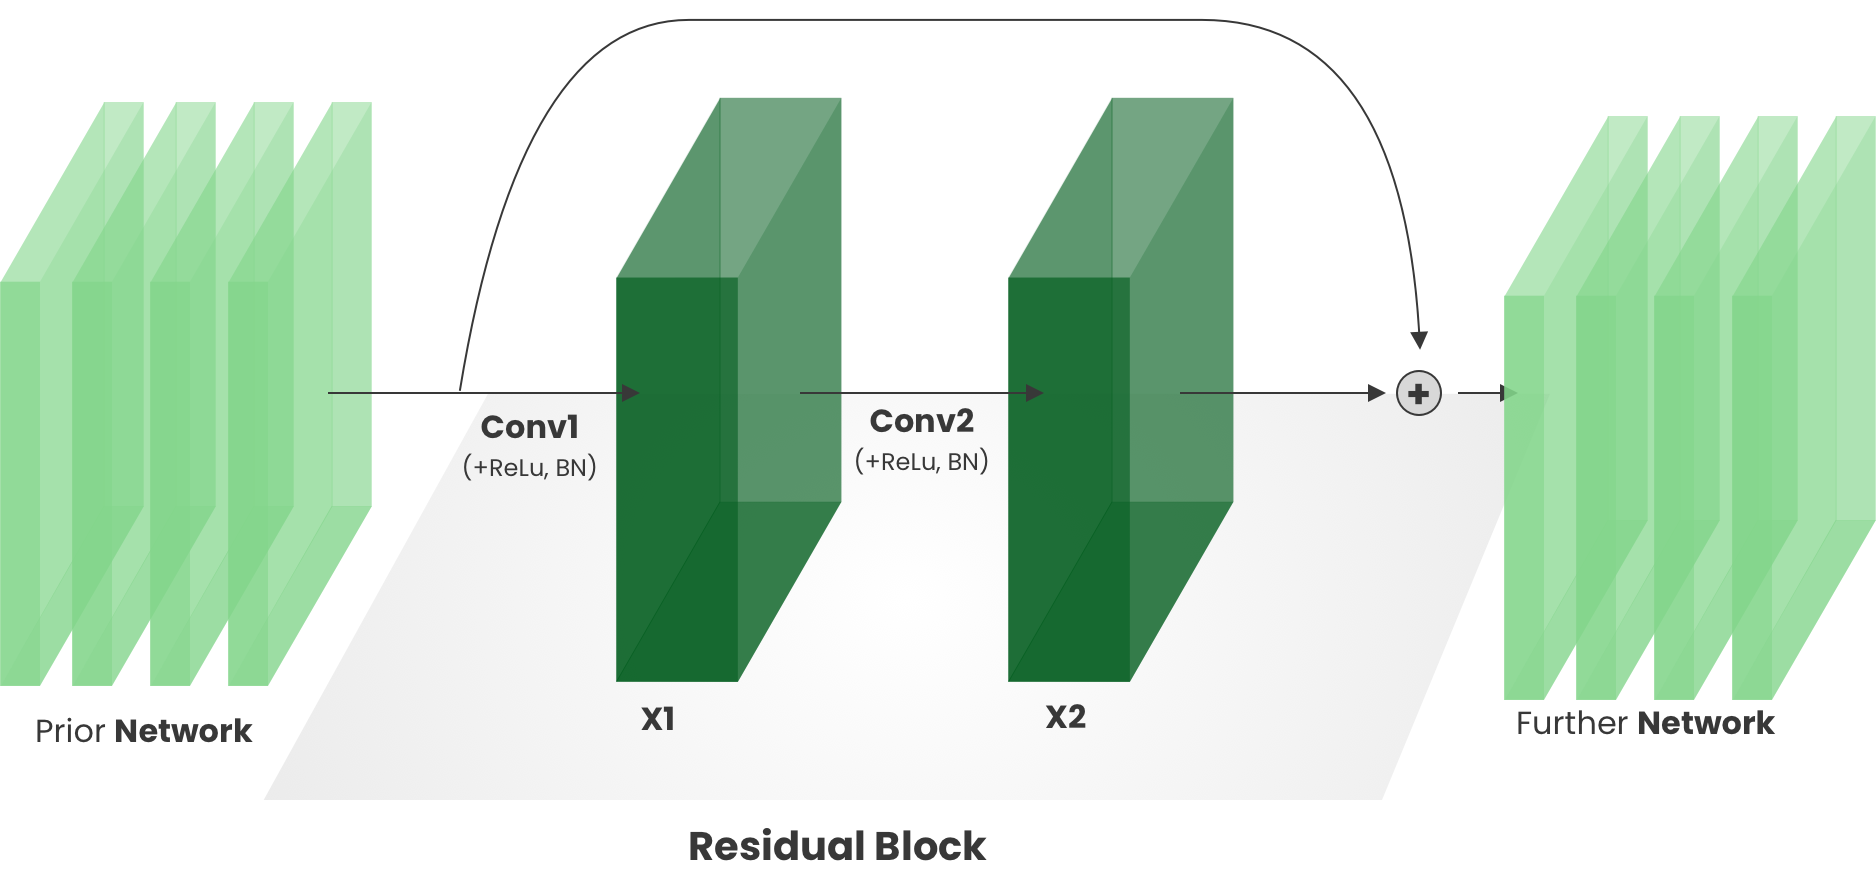
\includegraphics[width=0.8\textwidth]{./figures/resnet.png}
  \caption{\textbf{Residual Connection.} An illustration of a generic residual
  block, as defined by He \textit{et al.}~\cite{resnet}. A subnetwork of $L=2$ layers
  (consisting of convolution, batch normalization and ReLU layers) is applied to
  an input $x_0$. The first layer produces an output $x_1$, and the second layer
  an output $x_2$. The output of the residual block is given by $x_2+x_0$
  through the skip connection.
  }
  \label{fig:residual-connection}
\end{figure}

\textbf{DenseNets}~\cite{densenet} extend the idea of residual connections. At
the core of the DenseNet architecture is the concept of "dense blocks": Similar
to a residual block, it is a subnetwork of $L$ layers denoted as $H_l$. Unlike
the residual block, each layer in the dense block receives the concatenation of
all preceding layer outputs as an input, such that $x_l = H_l([x_0, x_1, \dots,
x_{l-1}])$. Dense blocks are compute intensive, but the strong connectivity
between layers support feature reuse, which allowed the architecture to be
shallower than predecessors. Again, the authors introduced several architectures
with different depths. Here, only DenseNet 121 is considered.

\begin{figure}
  \centering
  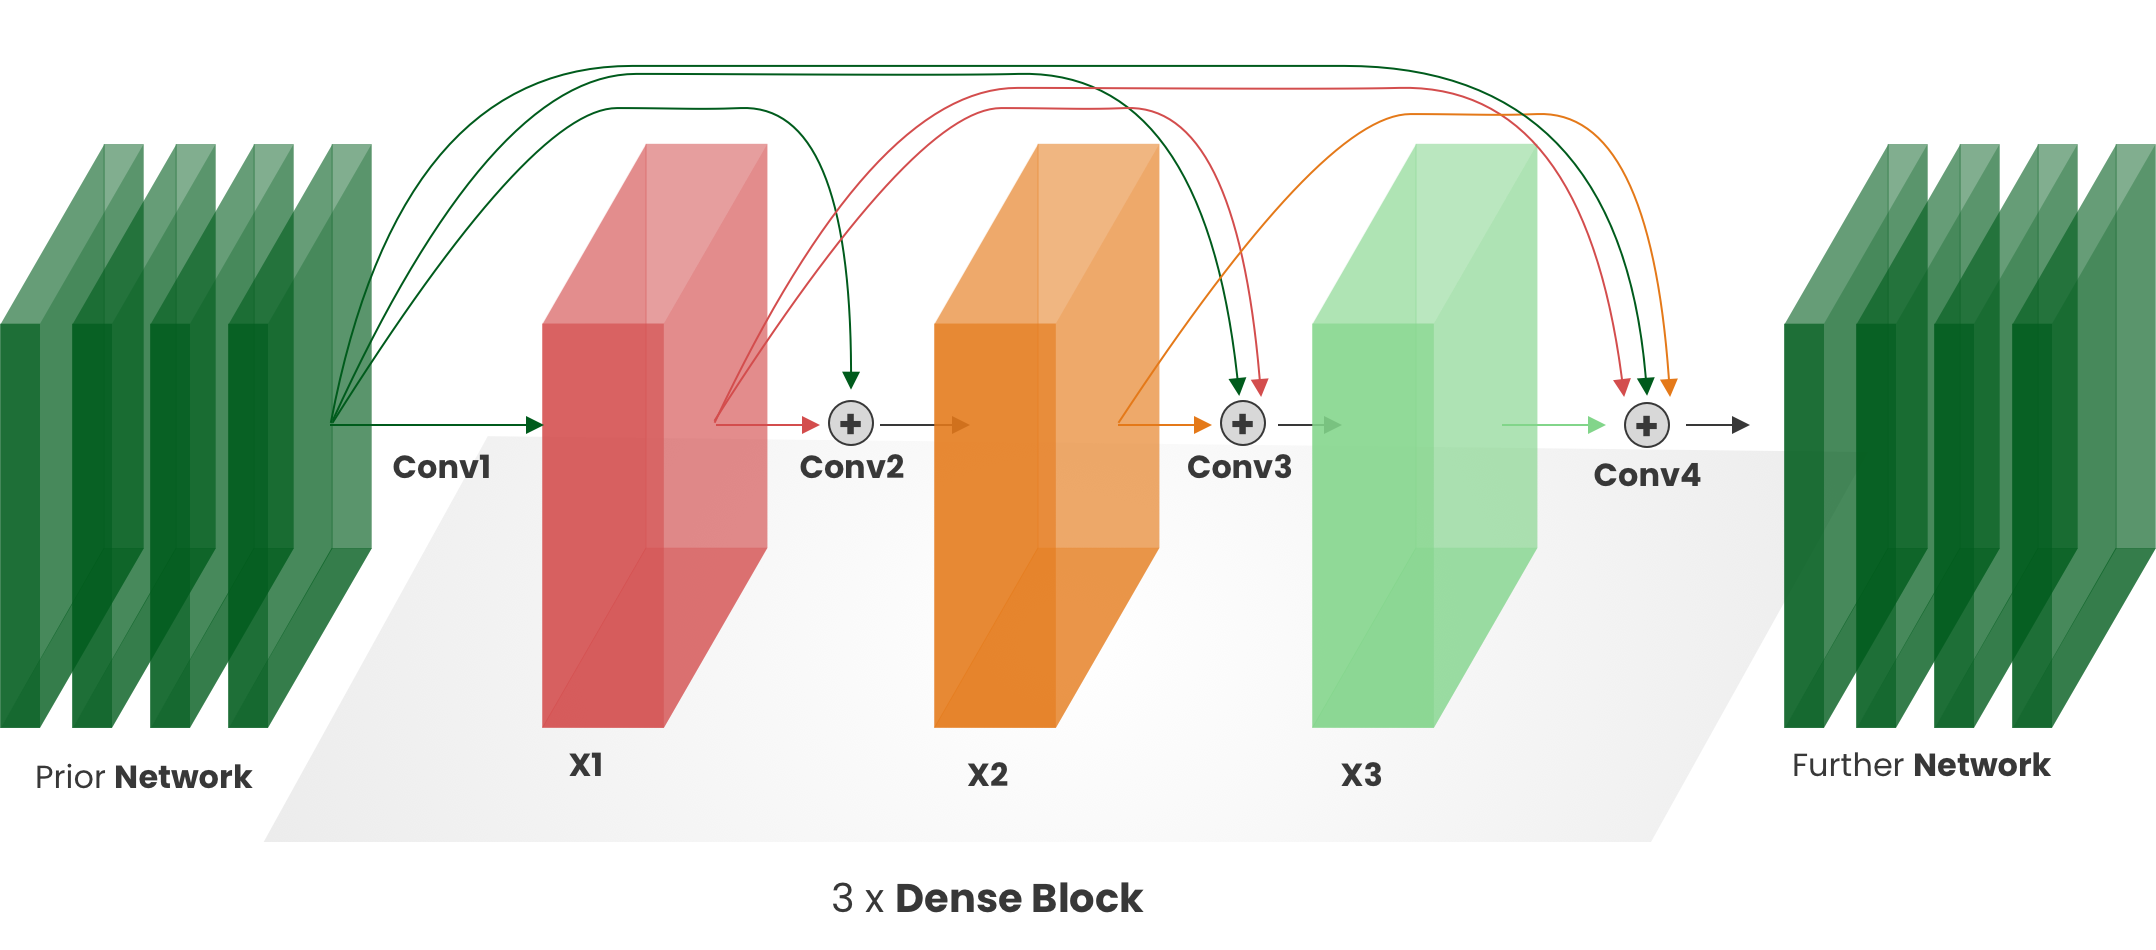
\includegraphics[width=.8\textwidth]{./figures/densenet.png}
  \caption{\textbf{Dense Block.} An illustration of a generic dense block, as
    defined by Huang \textit{et al.}~\cite{densenet}. A subnetwork of $L=4$ layers
    (consisting of convolution, batch normalization and ReLU layers) is applied
    to an input $x_0$. The $i$-th layer produces an output $x_i$. The input to
    the $i$-th layer is the concatenation of the output of all previous layers,
    so $H_i(x_i) = H_i([x_0, x_1, \dots, x_{i-1}])$. The final output of the
    denseblock is the concatenation of the output of all layers, so $x_4 = [x_0,
  x_1, x_2, x_3]$. }
  \label{fig:denseblock}
\end{figure}

\textbf{MobileNet V3}~\cite{mobilenetv3} is the third iteration of the MobileNet
architecture, which was introduced by Howard \textit{et al.} 2019. The main contribution
of MobileNets are so-called depth-wise separable convolutions. A depth-wise
separable convolution factorises a regular 2D convolution into two separate
steps: First, a single 2D filter is applied to each input channel separately,
and then a 1x1 convolution is applied to the output of the previous step. This
architectural change makes MobileNets significantly more efficient with only
minor performance losses, which made them popular for application on low-compute
devices, like mobile phones. MobileNet V3 is the most recent iteration of the
architecture, and its smallest variant, MobileNet V3 Small, is used in this
work.

\textbf{EfficientNet V2}~\cite{efficientnetv2}, proposed by Tan \textit{et al.}
in 2021, is searching for a compute-optimal CNN architecture. The main finding
of the paper is a scaling law, which states that for a given baseline network,
e.g. scaling up a network's depth, width and resolution with a constant factor
leads to improved performance and efficiency. In the original paper the authors
scale up previous state-of-the-art models like ResNet and MobileNet, which
showcase state-of-the-art performance, which make up a new family of models
called EfficientNets. Here, EfficientNet V2 S is used, which is the smallest
variant of the EfficientNet V2 family.

With the ground-breaking paper "Attention is all you need"~\cite{transformer},
Vaswani \textit{et al.} introduced the Transformer architecture in 2017.
Although being initially designed for machine translation, the architecture was
quickly adapted to other tasks in the domain of natural language processing,
superseding previous state-of-the-art models on various benchmarks. 

In 2020, \textbf{Vision Transformer}~\cite{vit} was introduced as one of the
first Transformer-based model adapted for the computer vision tasks. The main
contribution of the model is the patch embedding mechanism, which overcomes the
architectural mismatch between the two-dimensional input of images and the
one-dimensional input of Transformer architectures. Dosovitskiy \textit{et al.}
propose to split a 2d image into a sequence of fixed-sized patches, which are
then flattened and embedded into a sequence of "tokens". Together with
positional encodings for the position of the patch in the original image, this
sequence of tokens can be fed into a regular Transformer architecture. The
authors introduce several configuration of the architecture. In this work, the
base Vision Transformer, ViT-B-16, which is among the smaller variants of the
model is used.

Since then, many variants of the Vision Transformer have been proposed. They
either decrease the computational complexity of the architecture~\cite{deit,
vitlite}, or improve the performance by recovering some of the inherent
architectural advantages of convolutional neural networks~\cite{swin}. However,
these architectures are not considered in this work.

Finally, \textbf{ConvNext}~\cite{convnext} is one of the most modern
convolutional neural network architectures considered in this work and was
proposed by Liu \textit{et al.}~\cite{convnext} in 2021. Against the trend of
Transformer-based architectures in computer vision tasks, ConvNext is a pure
convolutional architecture. ConvNext uses the ResNet 50~\cite{resnet}
architecture as a baseline and performs gradual modernisation steps, ranging
from different optimisation algorithms, filter dimension to network depth and
width. The authors show that the resulting convolutional architecture is
competitive with the Transformer-based architectures, and coined in ConvNext.

\subsubsection{Video Classifiers} % (fold)

Early attempts of using 3D convolutional filters for video classification
tasks~\cite{i3d, c3d} show potential for modelling the temporal dimension of
video data. However, the authors also show that simple single-frame models
perform surprisingly well, and that the temporal dimension only provides
marginal gains. This finding and the fact that one would expect the temporal
information and motion patterns that emerge in sequences of images to be
important for video motivated Tran et. al to investigate different architectural
designs for video classification tasks. They contrast regular 2d convolution,
mixed 2d and 3d convolution, 3d convolution and 3d convolution with factorised
filters, which they coin \textbf{R(2+1)D}~\cite{r2plus1d}. They find that the
R(2+1)D architecture improves the performance on the Kinetics dataset by a
noticeable margin. 

In the same year, Feichtenhofer \textit{et al.}~\cite{slowfast} proposed
\textbf{SlowFast}~\cite{slowfast}, which introduces a two-stream architecture
for video classification tasks. SlowFast has two separate pathways for
processing video data. The first pathway, the slow pathway, processes the video
data at a low frame rate, which allows it to capture the spatial information of
the video data. The second pathway, the fast pathway, processes the video data
at a high frame rate, which allows it to capture the temporal information of the
video data. The authors show that the combination of the two pathways improves
the performance over single-stream architectures. In this study, both the
single-stream slow architecture \textbf{Slow R50} and the two-stream
architecture \textbf{SlowFast R50} are considered.

Finally, the \textbf{X3D} architecture reviews the design choices of previous
architectures that were proposed. The authors find that previous approaches
differ mainly by varying the temporal dimension (frame rate and number of
frames) and the spatial dimension (resolution, depth and width of filters).
Jointly studying the effects of scaling the temporal and spatial dimensions, the
authors propose a family of architectures that gradually scales up the depth,
width and resolution of the network, while keeping the computational complexity
constant. In this work, the smallest variant of the X3D family, X3D S,
is used.

% subsection models (end)

\subsection{Training} % (fold)
\label{sub:training}

All models were implemented using the deep learning framework
\texttt{PyTorch}~\cite{pytorch}. The model architectures were taken from the
\texttt{torchvision} and \texttt{pytorchvideo} libraries for single-frame and
video classification models, respectively and initialised with the default
pre-trained weights provided by the libraries. For all single-frame pre-training
was performed on the ImageNet dataset~\cite{imagenet} and for all video
classification models pre-training was performed on the Kinetics
dataset~\cite{kinetics}. Fine-tuning was then performed remotely on the high
performance cluster (HPC; Appendix~\ref{sub:machine-specs}) of the IT University
of Copenhagen using GPU-accelerated training. 

All models were optimised to minimise the cross-entropy loss function
$\mathcal{L}$ (Equation \ref{eq:cross-entropy}), 

\begin{equation}
  \mathcal{L}(\hat{\mathbf{y}},\mathbf{y}) = -\sum_{i=1}^{L} \mathbf{y}_i
  \log(\hat{\mathbf{y}}_i) \quad ,
  \label{eq:cross-entropy}
\end{equation}

% TODO: compare to pytorch cross-entropy loss (is it the same? what is the
% difference to nll?)

% TODO: models are all fine-tuned


where $\hat{\mathbf{y}}$ is the predicted probability distribution over the $L$
location labels and $\mathbf{y}$ is the one-hot encoded ground truth location
label for a single frame or video. The function penalises the model for
predicting a low probability for the ground truth label. For the models to learn
the relationship between frames/ clips and location labels, the gradient of the
loss function with respect to all model parameters is computed and
AdamW~\cite{adamw}, the de facto standard optimiser for deep learning models, is
employed to update the model parameters at a constant learning rate of
$10^{-4}$. No learning rate warm-up or scheduling was performed during training.

Mini-batch training was used for all models with a batch size of 16 for
single-frame models and 4 for video classification models due to memory
constraints. Because of the high computational complexity of 3D convolutions,
the video classification models take longer to converge and were therefore
trained for 15 epochs, while the single-frame models were trained for 10 epochs.

% \begin{table}
%   \caption{
%     \textbf{Default Training Hyperparameters.} The Table shows the default
%     hyperparameters for training the single-frame and video classification
%     models. The batch size is the number of samples that are processed in a
%     single forward and backward pass. The number of epochs is the number of
%     times the entire training dataset is passed through the model. The optimiser
%     is the optimisation algorithm used to minimise the loss function.}
%   \centering
%   \begin{tabular}{rlll}
%     \toprule
%     Classifier & Batch Size & Epochs & Optimiser \\
%     \midrule
%     \bfseries Single-Frame & 16 & 10 & AdamW ($\gamma=1e^{-4}$) \\
%     \bfseries Video & 4 & 15 & AdamW ($\gamma=1e^{-4}$) \\
%     \bottomrule
%   \end{tabular}
%   \label{tab:hyperparams}
% \end{table}

%   (end)

\subsection{Evaluation} % (fold)
\label{sub:evaluation}

To assess all models in terms of their performance and efficiency on the task
of location classification, a series of different performance and efficiency
metrics are computed. All metrics are computed on the test set, which was
separated from the original dataset before training, as described in
Section~\ref{sub:raw-data}.

\textbf{Quantifying Performance.} In the context of indoor location
classification, a model is considered to perform well if it is able to
accurately predict the location given a single frame or video clip. An intuitive
way to quantify the performance of a model is to compute the Top-K multi-class
accuracy:

\begin{equation}
  \text{Top-K Accuracy} = \frac{1}{N} \sum_{i=1}^{N} \mathbb{I}(y_i \in
  \mathcal{Y}_i) \quad ,
  \label{eq:top-k-accuracy}
\end{equation}

Here, $N$ is the number of samples, $y_i$ is the ground truth label for sample
$i$ and $\mathcal{Y}_i$ is the set of the top-k predictions for sample $i$. The
indicator function $\mathbb{I}$ is 1 if the ground truth label is in the set of
top-k predictions and 0 otherwise. Within the context of this report, the Top-1
and Top-3 accuracy are computed, which are measuring the ratio of samples for
which the true label is the top prediction, or within the top-3 predictions,
respectively.

Furthermore the Macro F1-score is computed. The F1 score is a class-specific
metric that measures the harmonic mean of precision and recall. The precision
$P_i$ of a classifier towards some class $i$ can be interpreted as the
probability that a sample that is classified as class $i$ is actually from class
$i$. The recall $R_i$ is the probability that a sample from class $i$ is
classified as class $i$. High precision and recall values are desirable, so an
ideal classifier would have a high precision and recall of 1. The F1-score is a
way to combine both metrics into a single metric by computing their harmonic
mean.

\begin{equation}
  P_i = \frac{TP_i}{TP_i + FP_i} \quad , \quad R_i = \frac{TP_i}{TP_i + FN_i}
  \quad , \quad F1_i = \frac{2 \cdot P_i \cdot R_i}{P_i + R_i} \quad ,
  \label{eq:f1-score}
\end{equation}

Finally, the Macro F1-score (Equation~\ref{eq:macro-f1-score}) is computed by
averaging the F1-scores for each location label.

\begin{equation}
  \text{Macro F1-score} = \frac{1}{L} \sum_{i=1}^{L} F1_i \quad .
  \label{eq:macro-f1-score}
\end{equation}

Here, each location label is weighted equally, regardless of the number of
samples that belong to the label. For the scope of this report the metric was
found to be a good extension to the Top-K accuracy, as it gives insights into
potential class imbalance issues.

\textbf{Quantifying Efficiency.} Efficiency is critical for real-time inference,
especially on mobile devices. For this reason, direct proxies for a model's
efficiency are computed using the \texttt{PyTorch Benchmark} library. The
library allows to track various metrics during inference on a single CPU. The
metrics that are computed are the mean inference time per sample (latency), the
mean number of samples per second (throughput), which are direct proxies for the
runtime of the model that can be expected when deployed.

\textbf{Understanding Model Behaviour.}  To understand the model behaviour in
more detail, the confusion matrix and a subset of the misclassified samples were
manually inspected for the best performing single-frame and video classification
model. 

% mention confusion matrix
A confusion matrix is a $L \times L$ matrix, where $L$ is the number of
location labels. The entry at index $(i,j)$ is the number of samples that were
predicted to belong to location label $j$, given the ground truth label $i$.
Confusion matrices are a traditional tool in classification tasks, as they give
a good overview of the models performance on the different classes and can
highlight regularly confused classes visually.

% mispredicted samples
Given the insights from the confusion matrix, a subset of the misclassified
samples was manually inspected, to understand why the model failed to predict 
the correct location label. This analysis should unveil what type of situations
are particularly challenging for the models and highlight potential areas for
improvement.

% real-time inference
Finally, the best performing single-frame and video classification model were
used to continuously predict the location label of a subset of the raw videos in
the test split to mimic a real-world deployment scenario. Again, the analysis 
of the results should drive focus to potential areas of improvement that are not
visible from looking at independent mispredicted samples.

% subsection evaluation (end)

% section methodology (end)

\section{Results} % (fold)
\label{sec:results}

% computer vision models are capable of solving indoor localisation when
% phrased as a classification task

Computer vision models, when carefully designed and trained, are generally
capable of providing reasonable accurate predictions on the task of indoor
localisation when phrased as a classification task. The detailed results of the
evaluation of the performance and efficiency of the different models are
presented in Table~\ref{tab:results} and discussed in the following.

\begin{table}
  \begin{tabular}{cllll|llll}
  \toprule
  & \multirow{2}{*}{\textbf{Model}} 
  & \bfseries Acc@1 & \bfseries Acc@3 & \bfseries Ma.-F1 & \bfseries FLOPs &
    \bfseries Latency & \bfseries Throughput \\
  & & (\%) & (\%) & (\%) & (G) & (ms/Pred) & (Preds/s) \\
  \midrule
  \multirow{8}{*}{\rotatebox[origin=c]{90}{Single Frame}}
  & AlexNet & 56.67 & 81.36 & 50.79 & 0.71 & 14.1 & 70.91 \\
  & Google LeNet & 63.40 & 84.74 & 56.80 & 1.97 & 47.2& 21.17 \\
  & DenseNet121 & 67.79 & 83.04 & 63.05 & 2.88 & 71.9 & 13.89 \\
  & ResNet18 & 70.65 & 89.73 & 64.84 & 1.82 & 27.1 & 37.22 \\
  & ResNet 50 & 55.76 & 77.65 & 50.05 & 4.12 & 60.9 & 16.41 \\
  & MobileNet V3 Small & 28.68 & 51.34 & 19.21 & 0.06 & \bfseries 11.9 & \bfseries 83.82 \\
  & ViT B-16 & 53.20 & 77.57 & 47.54 & 17.59 & 166.0 & 6.03 \\
  & EfficientNet V2 Small & 50.51 & 81.73 & 41.71 & 2.88 & 77.6 & 12.91 \\
  \midrule
  \multirow{2}{*}{\rotatebox[origin=c]{90}{Video}}
  & R(2+1)D & \bfseries 78.33 & \bfseries 91.67 & \bfseries 75.27 & \bfseries 93.72 & 825.1 & 1.22 \\
  & X3D & 68.89 & 81.11 & 54.09 & 2.85 & 229.0 & 4.37 \\
  \bottomrule
  \end{tabular}

  \caption{ 
    \textbf{Results.} The table the performance and efficiency metrics for all
    trained models. The models are grouped by their type (single-frame or
    video). The performance metrics are the top-1 accuracy (Acc@1), top-3
    accuracy (Acc@3) and Macro F1-Score (Ma.-F1). The efficiency metrics are
    the number of floating point operations (FLOPs) per inference, the mean
    inference time in milliseconds per prediction (Latency) and the mean
    number of predictions per second (Throughput). The best performing model
    in each category is highlighted in bold. The metrics are computed on the
    test set of the respective dataset. 
  }
  \label{tab:results} 
\end{table}

\subsection{Detailed Analysis of Single-Frame Classifiers} % (fold)
\label{sub:analysis-single-frame-classifiers}

% single-frame classifiers are capable of solving the task
Surprisingly, even simple single-frame classification models are capable of
providing a reasonable solution to the task of indoor localisation. Despite
the lack of information about the temporal context of the frames, the
best-performing single-frame classifier (ResNet18) achieves a top-1 accuracy
of 70.65\% and a top-3 accuracy of 89.73\%. This is a significant result as it
shows that processing single frames of the video is sufficient to solve the
task of indoor localisation. This is especially important in the context of
mobile devices, and applications where real-time inference is required.

% single-frame classifiers are efficient
Out of the single-frame classifiers, three classifiers can produce real-time
predictions on a mobile device, as they have a higher throughput rate than
video frame rate. The most efficient model is MobileNet V3 with a throughput of
83.82 predictions per second. AlexNet and ResNet18 are also capable of
real-time inference with throughputs of 70.91 and 37.22 predictions per
second, respectively. All other models are not capable of real-time inference
on a mobile device, but are sufficiently quick to provide near real-time
predictions.

% model complexity vs. performance
Evidence in computer vision research suggests that more complex models
typically are able to achieve better performance. This is not entirely the
case for this study. The smallest model, MobileNet V3, is a clear outlier in
terms of performance, only achieving a top-1 accuracy of 28.68\%. It is
hypothesised that the model is not complex enough to handle the challenging
20-class classification task. As models are getting more complex, the
performance increases up until the complexity of ResNet18 (11.2M parameters).
All models with a higher number of parameters than ResNet18 perform worse.
Interestingly, the most complex model in terms of the total number of
parameters, ViT-B-16 (85.8M), which achieves state-of-the-art results on
common image classification benchmarks, is not the best-performing model in
this study. This is likely due to the small size of the dataset in combination
with relatively few training epochs. 

% end subsection analysis-single-frame-classifiers

\subsection{Detailed Analysis of Video Classifiers} % (fold)
\label{sub:detailed-analysis-of-video-classifiers}

As the nature of the task is inherently temporal, it is not surprising that
video classifiers outperform single-frame classifiers
(Figure~\ref{fig:performance-metrics}). The best performing video classifier is
R(2+1)D with a top-1 accuracy of 78.33\% and a top-3 accuracy of 91.67\%. This
is a significant improvement over the best performing single-frame classifier,
ResNet18. The video classifiers are more robust to noise in the input data, as
they are able to leverage the temporal context of the video. For example, the
model is capable of predicting a clip correctly despite a few frames being
occluded by a person walking through the scene or other sources of noise. This
capability has proven especially useful in the context of indoor localisation,
as high variation in the environment and therefore high noise in the input
data is common.

% video classifiers are less efficient
Video classifiers generally require more compute and memory resources during
inference, as they have to keep a history of the previous frames in memory.
This is reflected in the efficiency metrics. R2+1D has a throughput of only
1.22 predictions per second. This means that it can only provide predictions
for the location every second. This makes the model slower in responding to
sudden changes in the environment.

% subsection detailed analysis of video classifiers (end)

\begin{figure}
  \begin{center}
    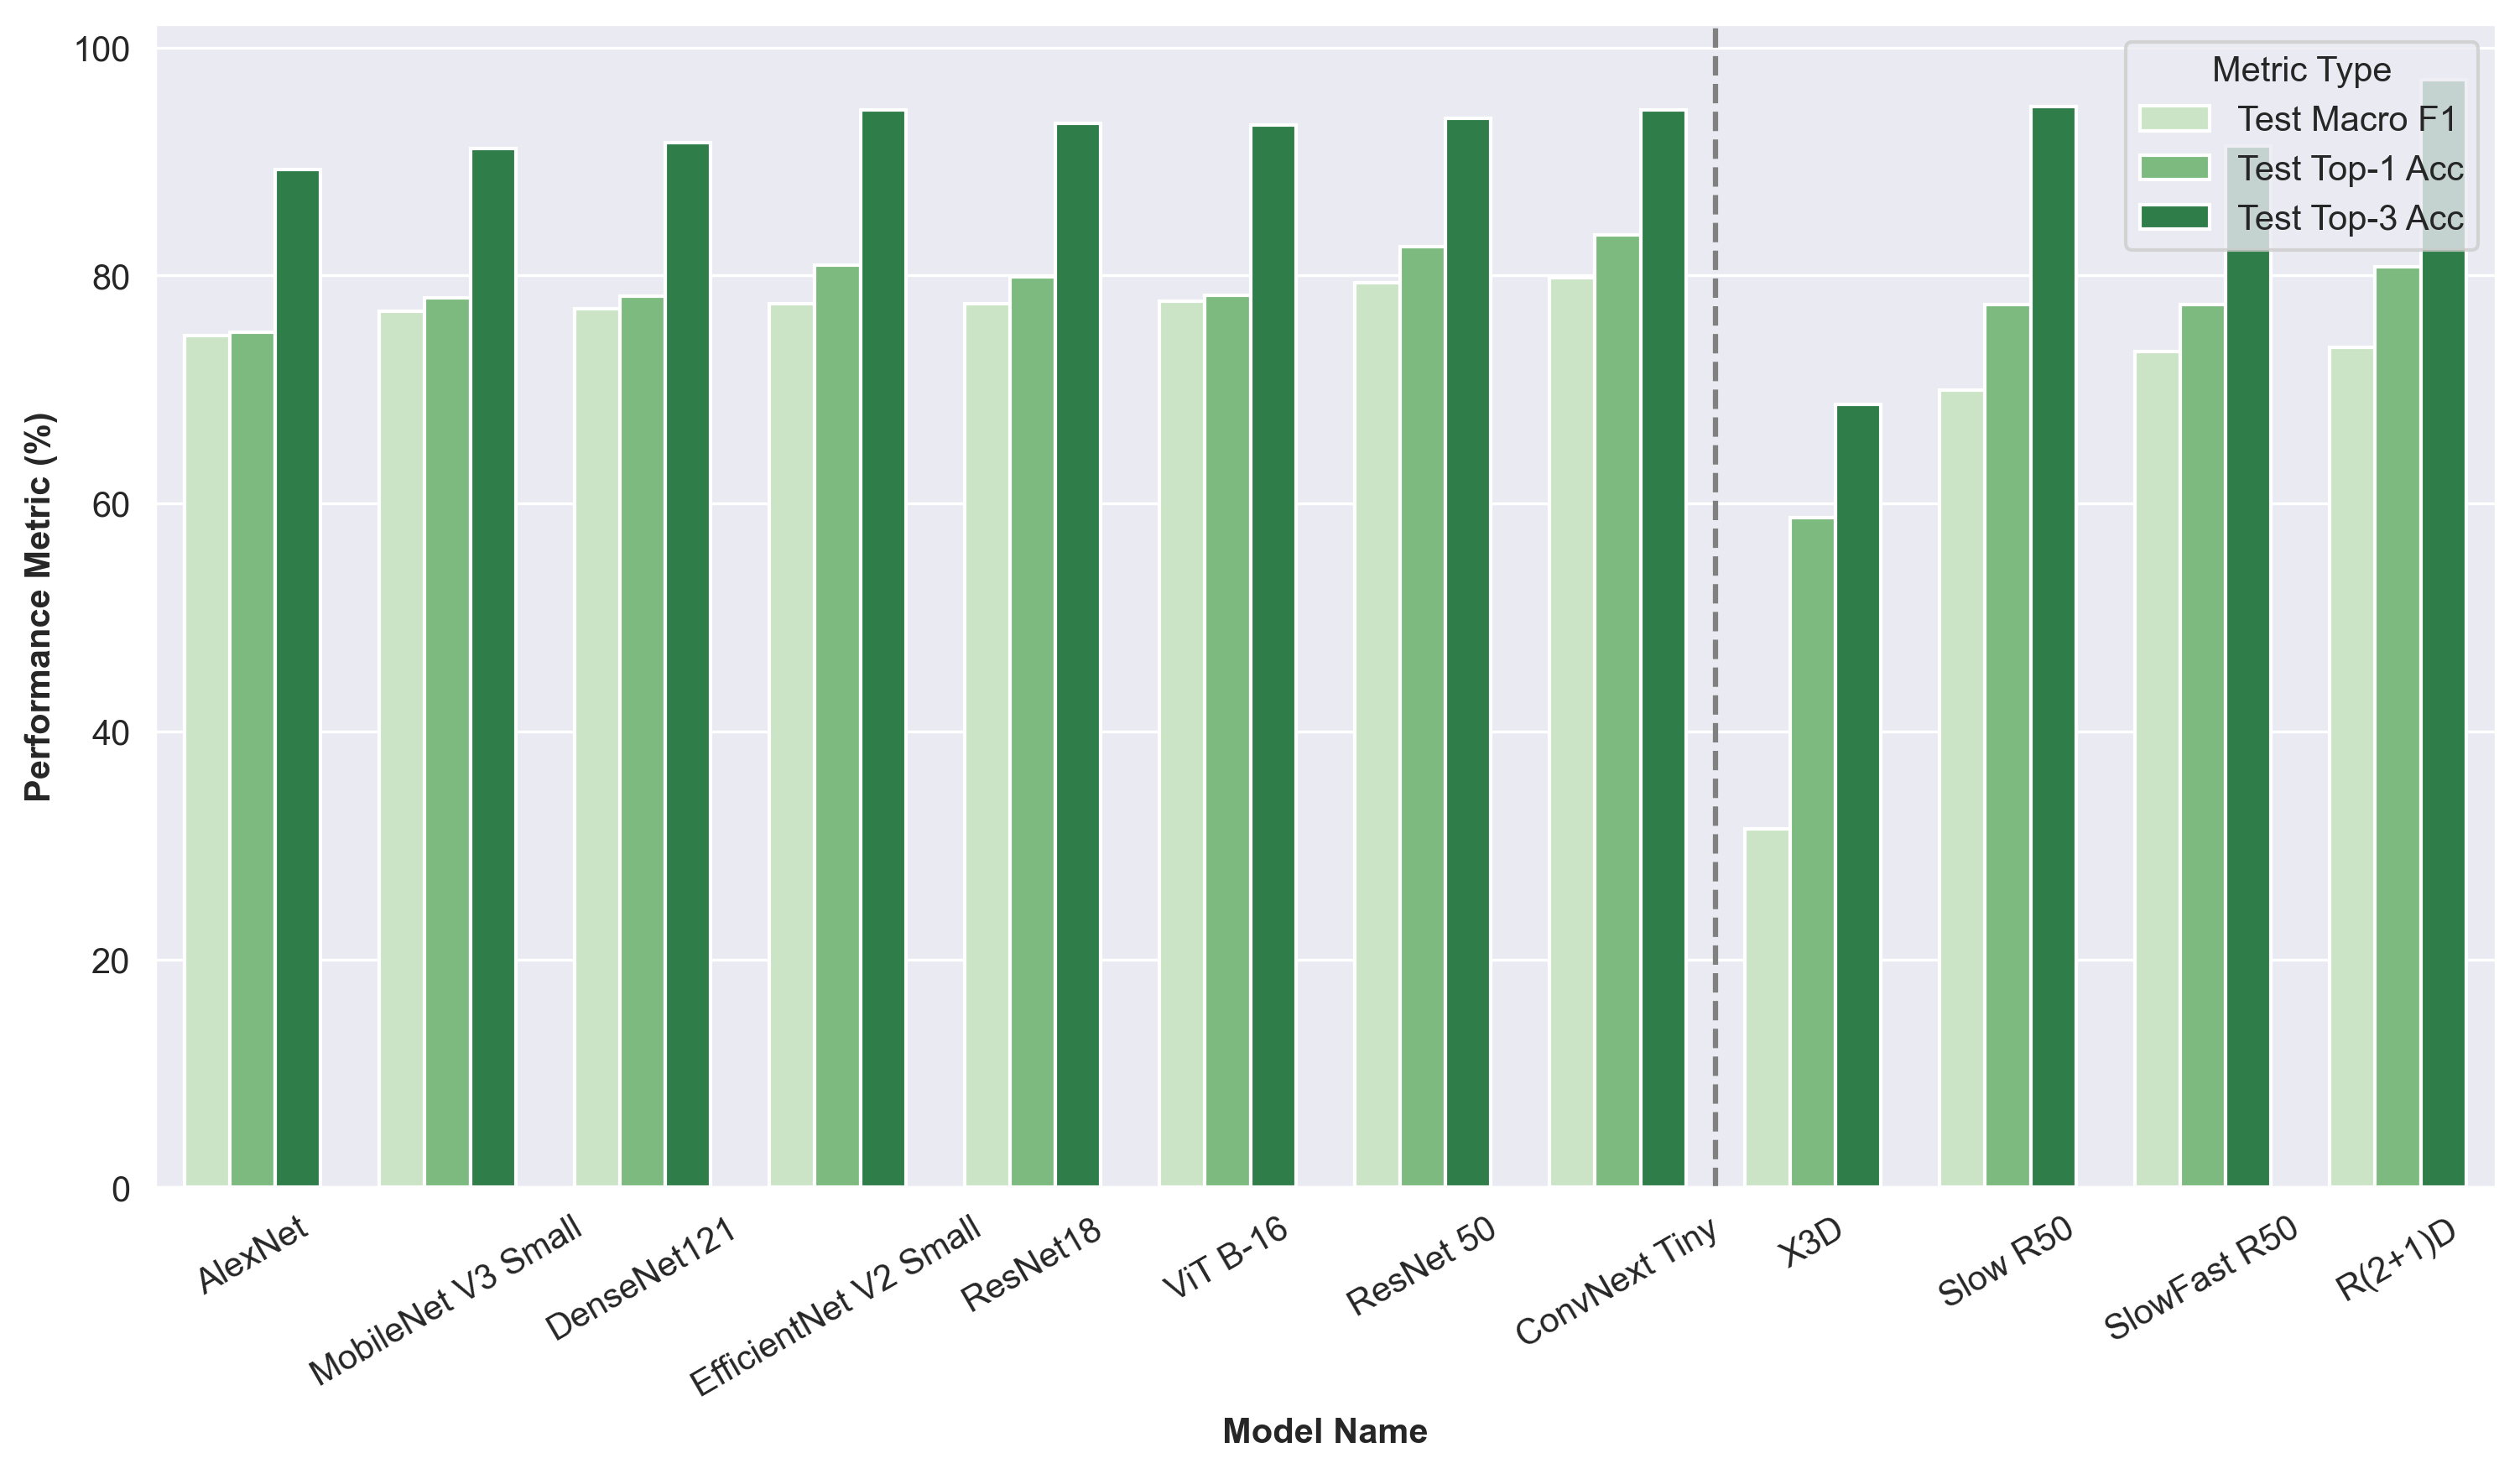
\includegraphics[width=.95\textwidth]
    {./figures/performance-metrics.png}
  \end{center}

  \caption{\textbf{Performance Metrics.} The Figure shows the performance
    metrics, Macro F1, Top-1 Accuracy and Top-3 Accuracy, for all trained
    models on the test split. A grey, dotted line separates the single-frame
    classifiers (left) from the video classifiers (right). Within their group,
    models are sorted from left to right by their Top-1 Accuracy.}

  \label{fig:performance-metrics}
\end{figure}

\subsection{Performance Efficiency Trade-Off} % (fold)
\label{sub:tradeoff}

The pre-dominant tendency in deep learning is that with sufficient data sizes
and compute resources, more complex models outperform simpler ones. However,
there is a trade-off between model complexity and efficiency, when inference
time is critical like when deployed on a mobile device. 

Figure~\ref{fig:tradeoff} shows the Top-1 Test Accuracy of all models against
latency (left) and throughput (right). Latency and throughput are meaningful
metrics to assess model's efficiency, as they are a direct proxy for the
real-time inference speed when deployed on low-resource device. While the
benchmarks were computed on a desktop CPU, they give a good indication of the
relative performance of the models and allow to extrapolate the insights to
performance on a mobile device. It is to be noted that latency and throughput
are inversely proportional to each other: Less inference time per sample (low
latency) leads to a higher number of inferences per second (high throughput).
However, as inference times vary greatly between models, the two metrics are
plotted separately, as they highlight different tails of the distribution.
Specifically, the latency plot accentuates high latency models, while the
throughput plot highlights low latency models.

% latency-accuracy
In Figure~\ref{fig:tradeoff}a, R(2+1)D is a clear outlier. The model has the
highest latency, but also the best overall performance. The increase in
complexity over X3D seems to be justified, as the model achieves a 9.4\%
increase in Top-1 Accuracy, while only increasing the latency by 0.6 seconds.
A similar trend cannot be observed for the single-frame classifiers. As
latency times are close to each, their trend is easier to study in
Figure~\ref{fig:tradeoff}b. Here, a quadratic relationship between throughput
and accuracy can be observed for the single-frame classifiers.
High-complexity, but low-throughput models, like ViT-B-16, EfficientNet V2 S
and ResNet18 are outperformed by lower-complexity models. Similarly,
low-complexity, but high-throughput models, like MobileNet V3 and AlexNet,
show similarly low performance. The sweet spot in terms of throughput and
accuracy is ResNet18, which achieves a throughput of 37.22 predictions per
second and a top-1 accuracy of 72.92\% This phenomenon is best explained by
the fact that low-complexity models are not able to capture the complexity of
the task, while high-complexity models are not able to learn from the small
dataset. The video classification models defy this trend, as they are all
low-throughput, but high-performing.

\begin{figure}
\centering
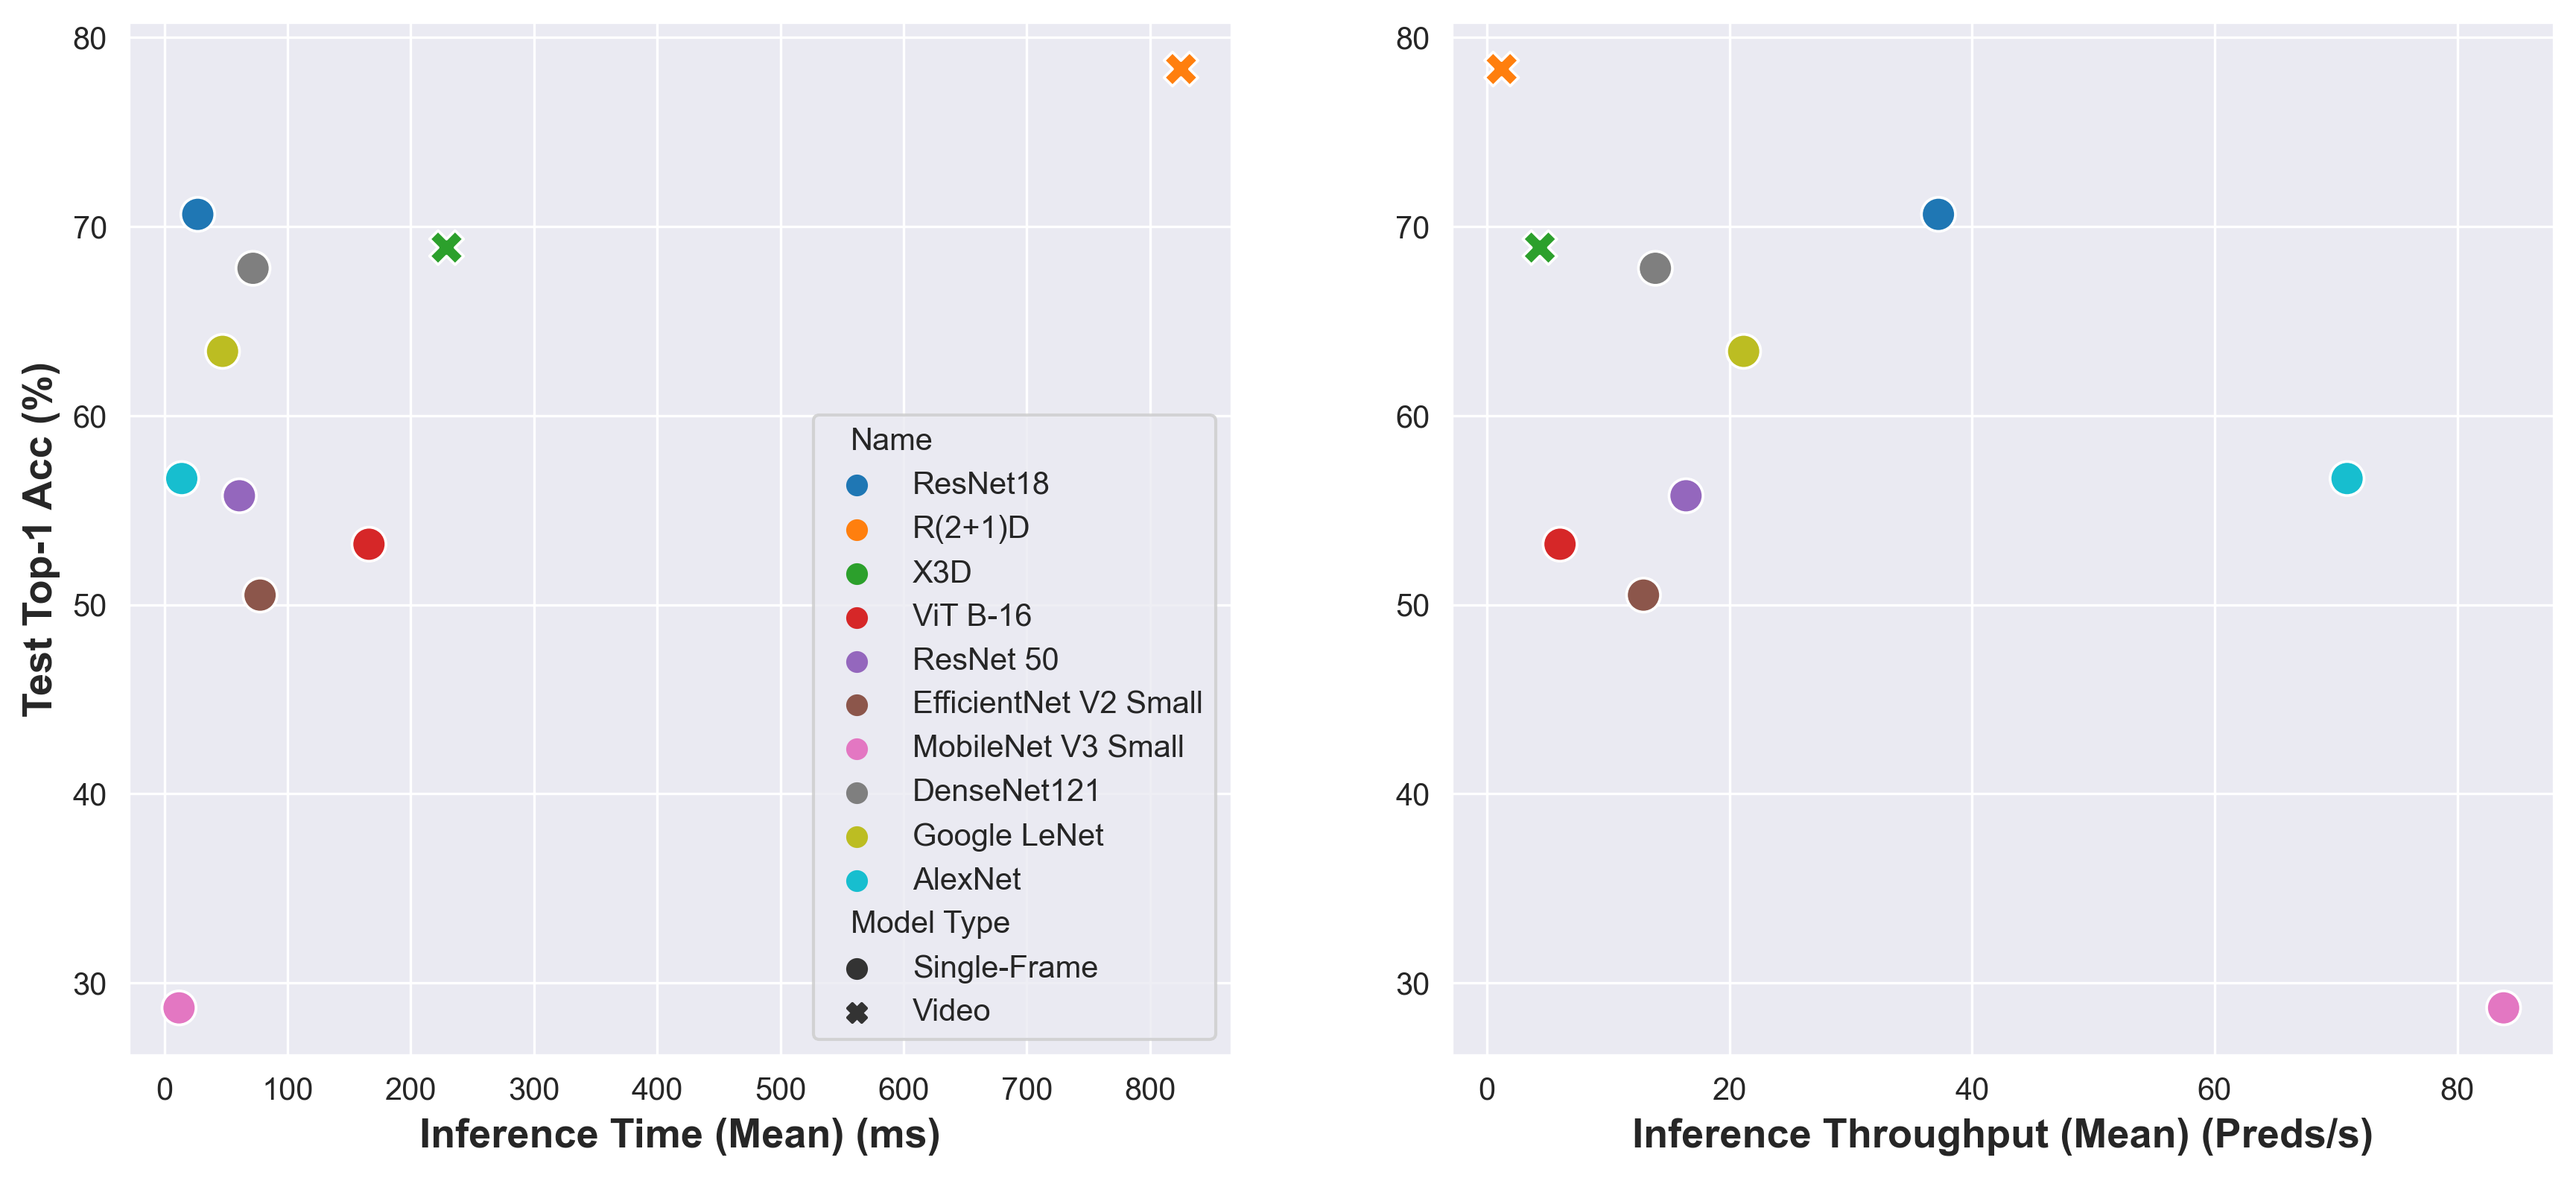
\includegraphics[width=\textwidth]{
./figures/performance-efficiency-tradeoff-scatter.png}
\caption{
  \textbf{Performance-Efficiency Trade-Off.} The Figure visualises the
  performance-efficiency trade-off for all models by plotting the
  relationship between the Top-1 Accuracy against the latency (inference
  time in milliseconds per prediction) and throughput (predictions per
  second). Each model is given unique colour, and the marker type indicates
  whether the model is a single-frame classifier (circle) or a video
  classifier (cross).
}

\label{fig:tradeoff}
\end{figure}

% subsection tradeoff (end)

\subsection{Analysing Prediction Patterns: Confusion Matrices} % (fold)
\label{sub:conf-matrices}

To better understand the strengths and weaknesses of deep learning models in
tackling the task of indoor classification, the two best performing models,
ResNet18 and R(2+1)D, are analysed in more detail. Specifically, the confusion
matrices of the two models are analysed to identify common failure modes of
the models.

Figure~\ref{fig:conf-matrix} shows the confusion matrices for (a) ResNet18 and
(b) R(2+1)D. It becomes clear that both models struggle with the same
misclassification scenarios. The most common misclassification is between the
two corridors on the ground floor (\textit{Ground Floor Corridor 1} and
\textit{Ground Floor Corridor 2}) and the Atrium (bottom-right grey
rectangle). ResNet18 both confuses the two corridors and has a tendency for
predicting the majority class (Atrium) instead of Corridor 2. R(2+1)D rarely
confuses the corridor, but has an even stronger tendency for predicting
Corridor 2 as Atrium. These failure cases are explained by the fact that the
two corridors and the Atrium are visually very similar. Furthermore, they are
directly adjacent to each other, which likely leads to some naturally
occurring failure cases at the border of the areas. Here, the model might
predict the new class earlier or later than the ground truth label changes.

Another region with similar behaviour are the three libraries on the first
floor (\textit{First Floor Library}, \textit{First
Floor Library 2}, \textit{First Floor Library 3}). Especially ResNet18
struggles to distinguish between the three classes, which is understandable
given the fact that the dominating visual feature of the three classes are 
rows of bookshelves. R(2+1)D shows a similar, but less pronounced behaviour.
One explanation might be that while the shared visual feature of bookshelves,
the arrangement of the bookshelves is different in the three libraries, which
can be learned by R(2+1)D due to its temporal modelling capabilities.

\begin{figure}
  \centering
  \begin{subfigure}[b]{0.49\textwidth}
    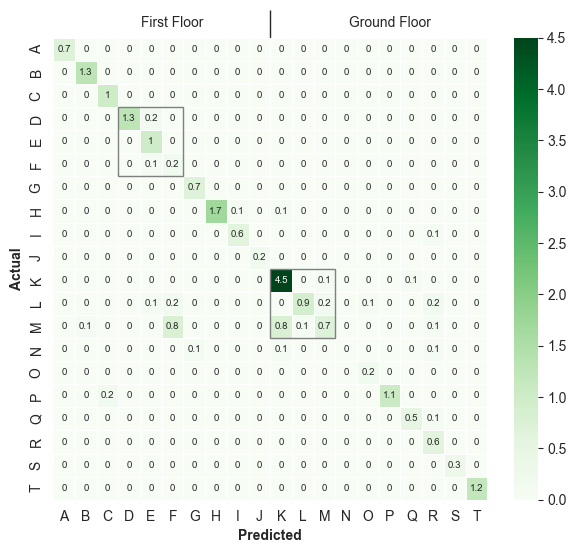
\includegraphics[width=\textwidth]{./figures/conf-matrix-resnet18.png}
    \caption{ResNet18}
  \end{subfigure}
  \begin{subfigure}[b]{0.49\textwidth}
    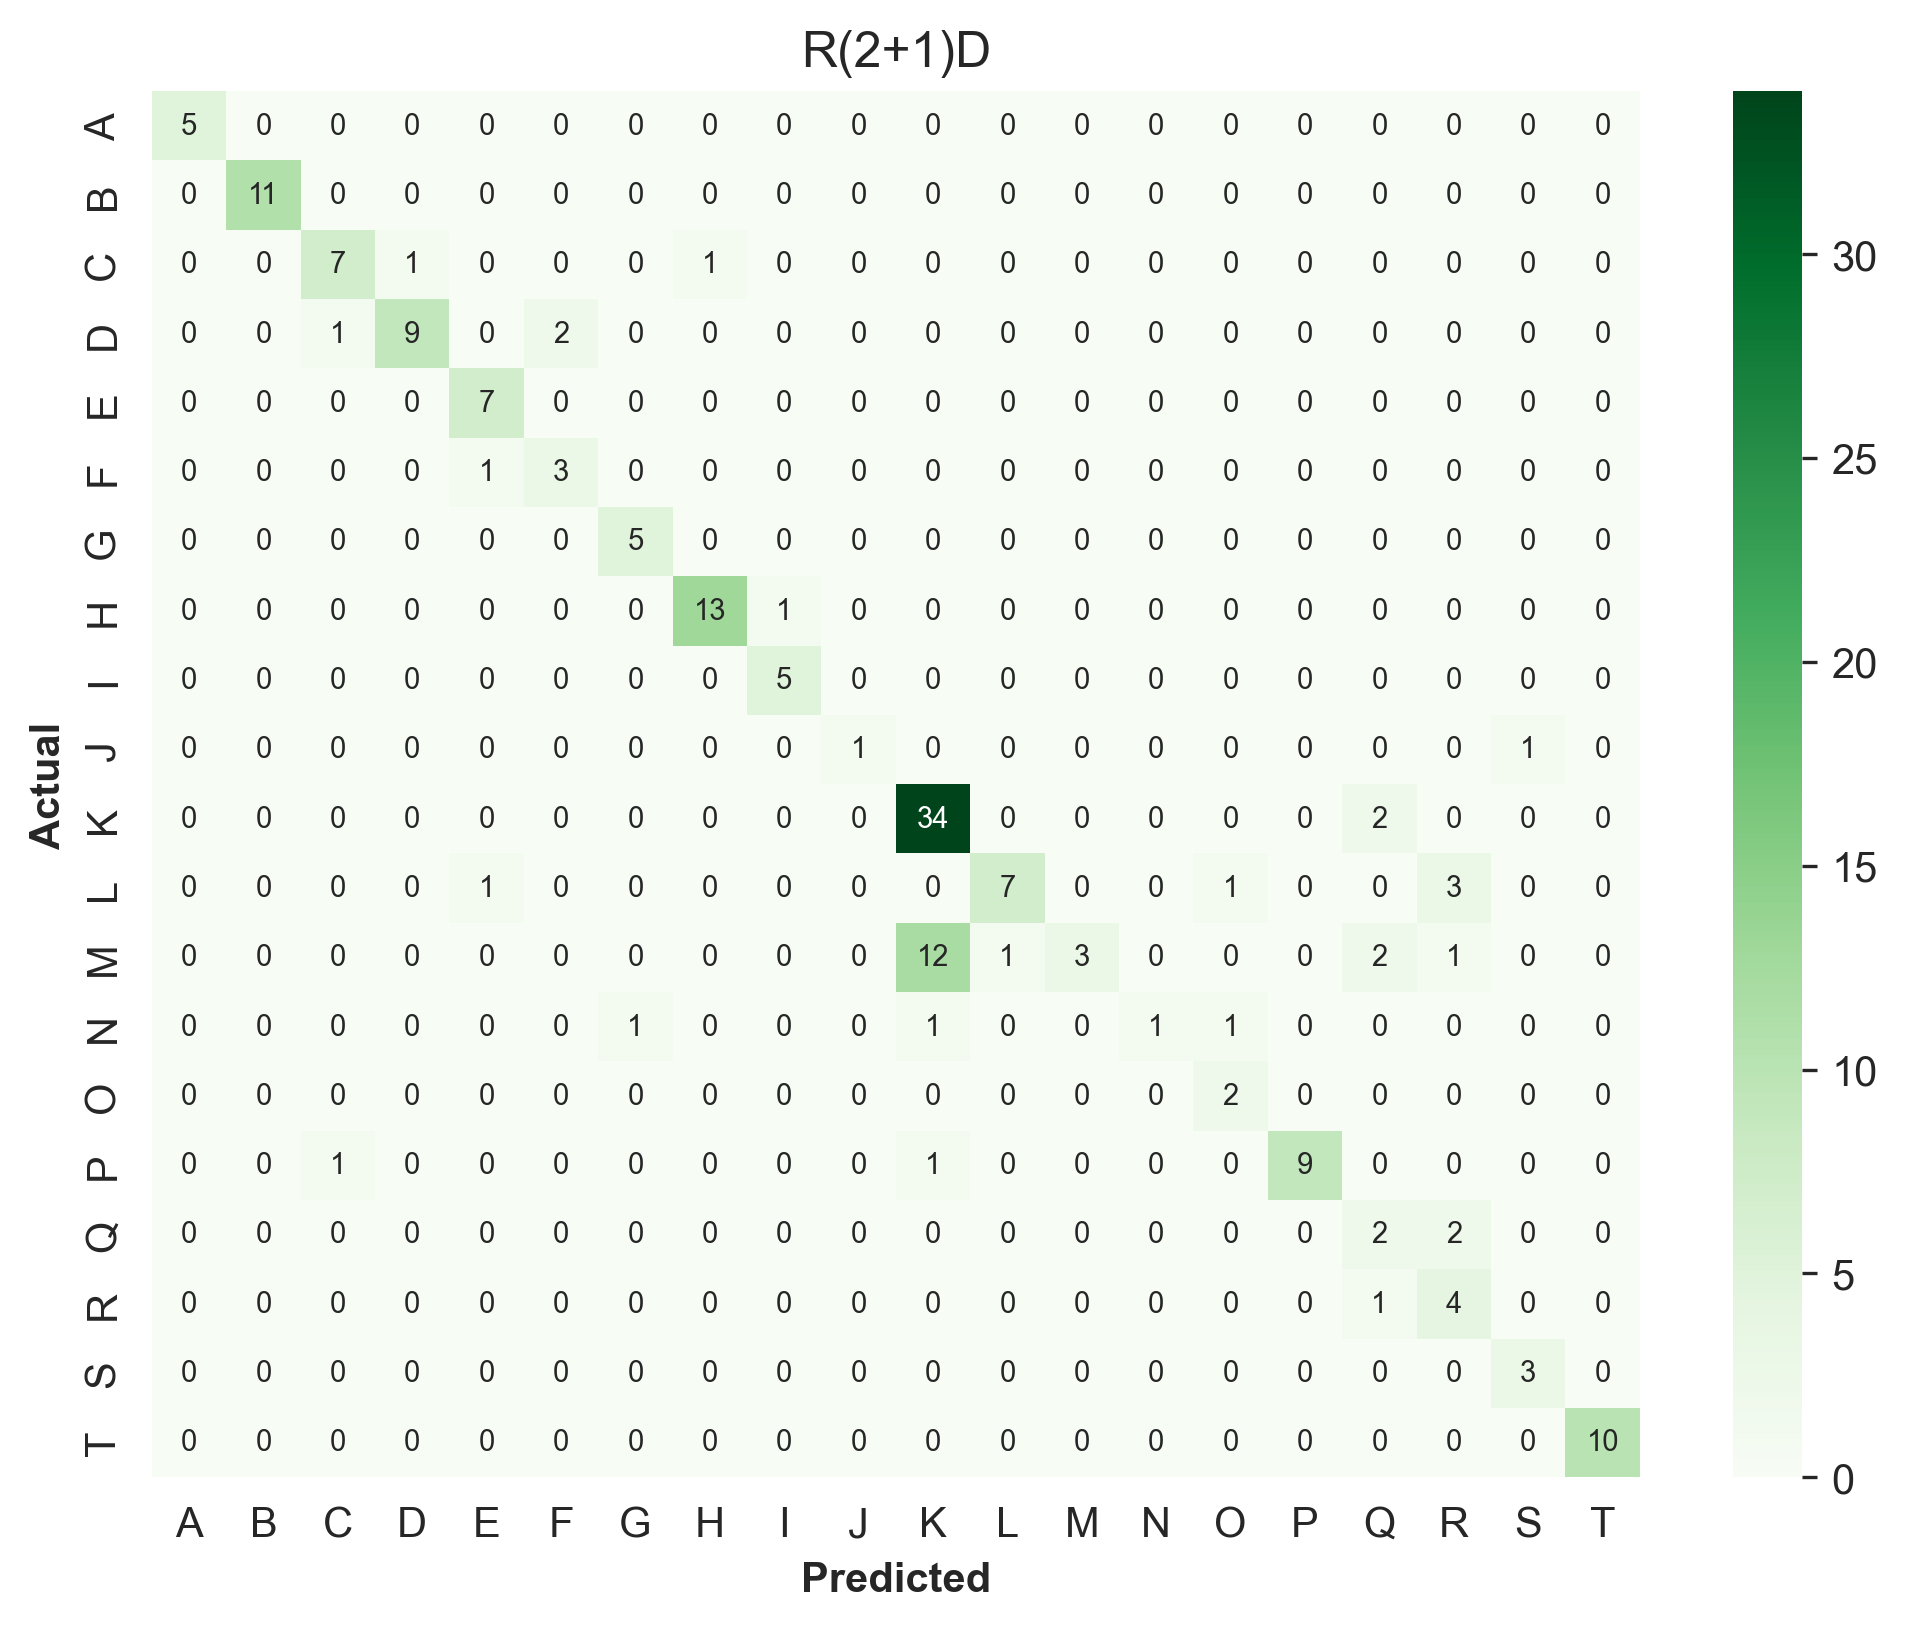
\includegraphics[width=\textwidth]{./figures/conf-matrix-r(2+1)d.png}
    \caption{R(2+1)D}
  \end{subfigure}
  \caption{
    \textbf{Confusion Matrices.} The Figure shows the confusion matrix for (a)
    ResNet18 (best performing single-frame classifier) and (b) R(2+1)D (best
    performing video classifier). The confusion matrix of ResNet18 is
    normalised to show 1K samples per class for visual purposes. For both
    matrices, the entry at row $i$ and column $j$ shows the number of samples
    that belong to class $i$ but were predicted to be class $j$. Gray
    rectangles indicate challenging classes, that are often confused.
  }
  \label{fig:conf-matrix}
\end{figure}

% TODO: add conf matrices with classes ordered by ground/ first floor
% similarity

\subsection{Analysing Failing Scenarios: Mispredicted Samples} % (fold)
\label{sub:mispredicted}

Figure~\ref{fig:mispredicted} shows three exemplary mispredicted samples for
(a) ResNet18 and (b) R(2+1)D. The respective legend shows the top 3 predicted
classes for each sample in order of confidence and the ground truth label. 

For ResNet18, the first sample shows a misclassification between the two
corridors on the ground floor, which is the most common misclassification for
ResNet18 as seen from the confusion matrix (Figure~\ref{fig:conf-matrix}a). It
can be seen, that the model is unsure about the prediction (64\% confidence in
Corridor 2 and 34\% confidence in Corridor 1). The second and third sample
show another common misclassification mode. Here the model confuses the 
the yellow and green area on the ground and first floor, respectively.

For R(2+1)D, the first sample shows a transition misprediction. The frame is
directly at the border between the Magenta Area and Corridor 2 on the ground
floor and predicts the Magenta Area, while the ground truth label is Corridor
2. The second sample shows a truly sample from a challenging video from the
test split, because the video shows an area that was freshly painted in blue
in Corridor 2. As the training split does not contain any videos from this
area, the model has never seen this area in blue and thus predicts a wrong
area, in this case the majority class Atrium. The third sample shows another 
misprediction of similar classes. The clip starts at the very end of the
entrance with the camera facing to the outside. The model predicts the yellow
entrance, when the ground truth label is the magenta entrance.


\begin{figure}
\centering

\begin{subfigure}[b]{\textwidth}
\centering
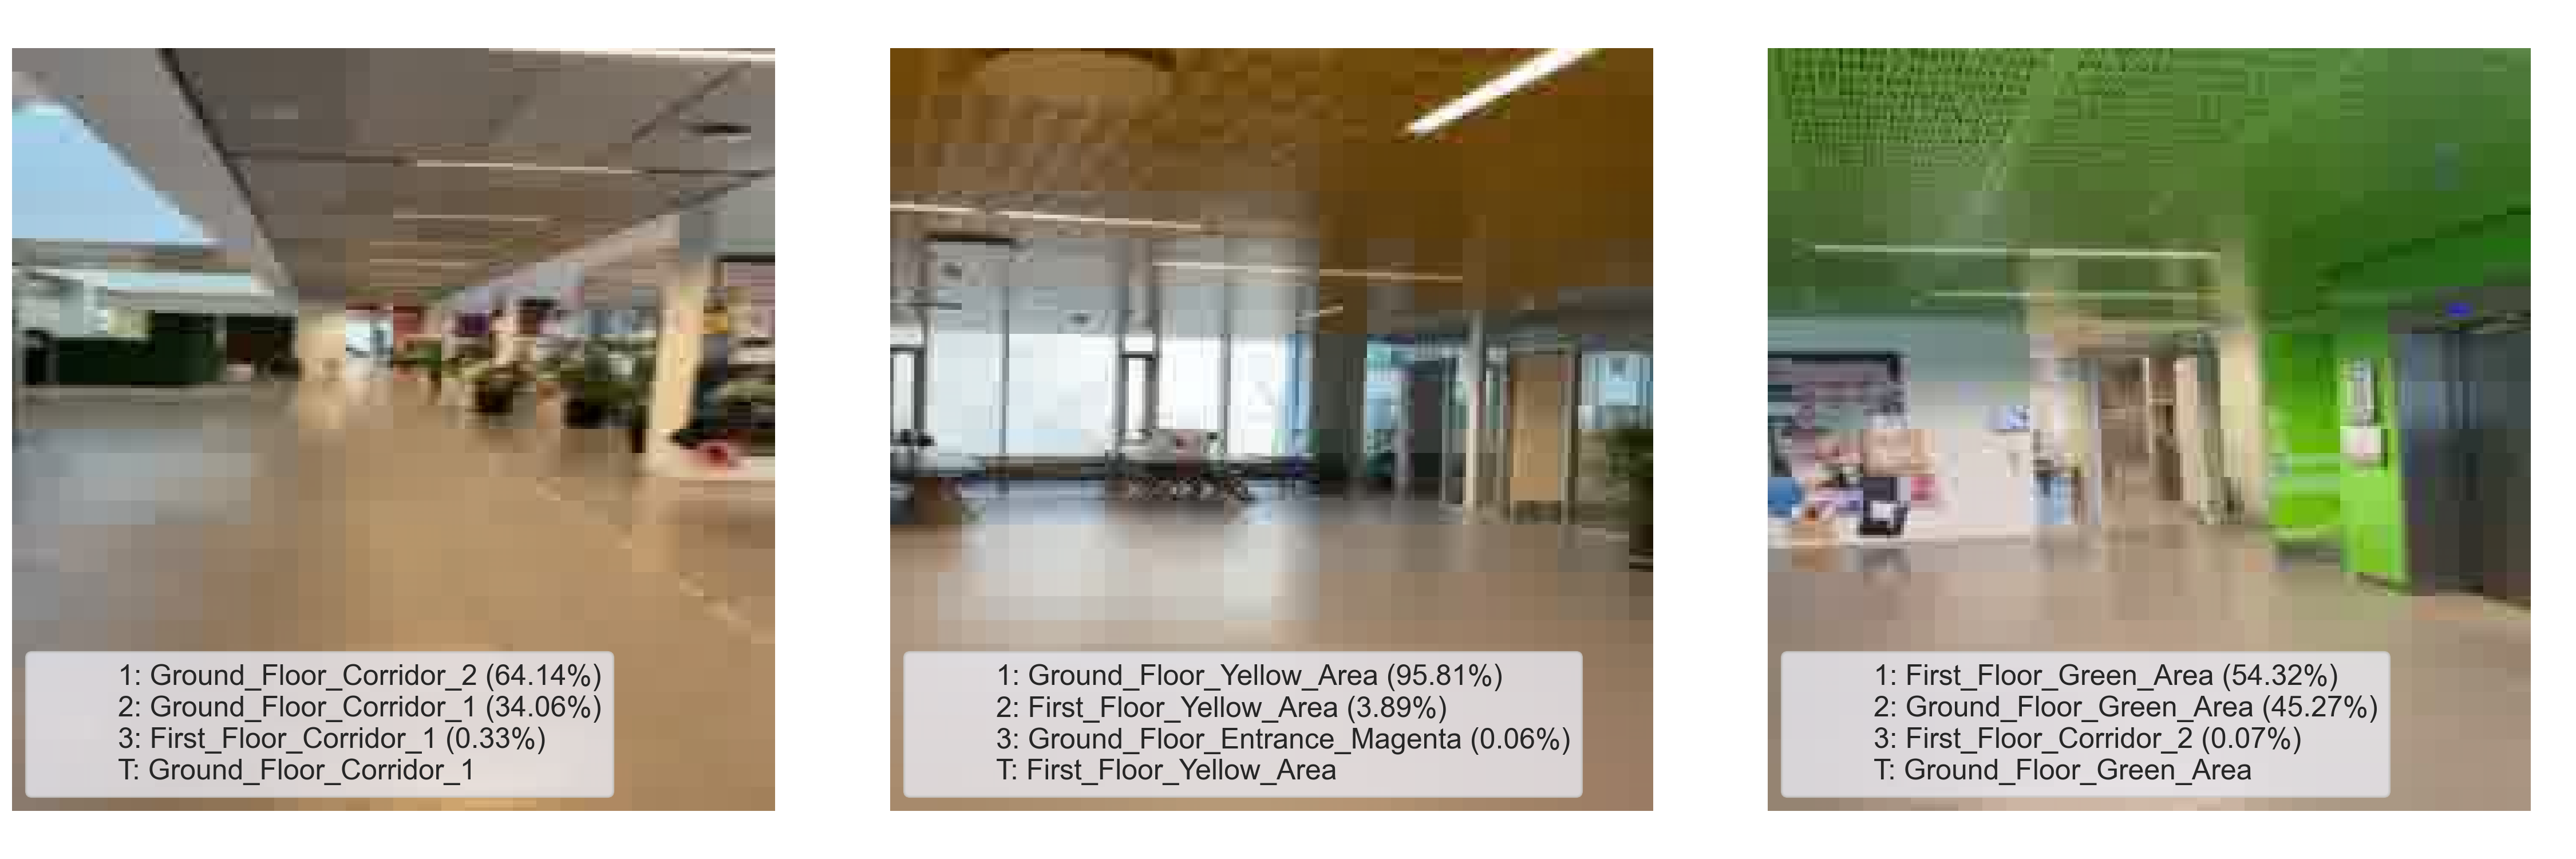
\includegraphics[width=\textwidth]{./figures/resnet18-mispredicted-frames.png}
\caption{ResNet18}
\end{subfigure}

\begin{subfigure}[b]{\textwidth}
\centering
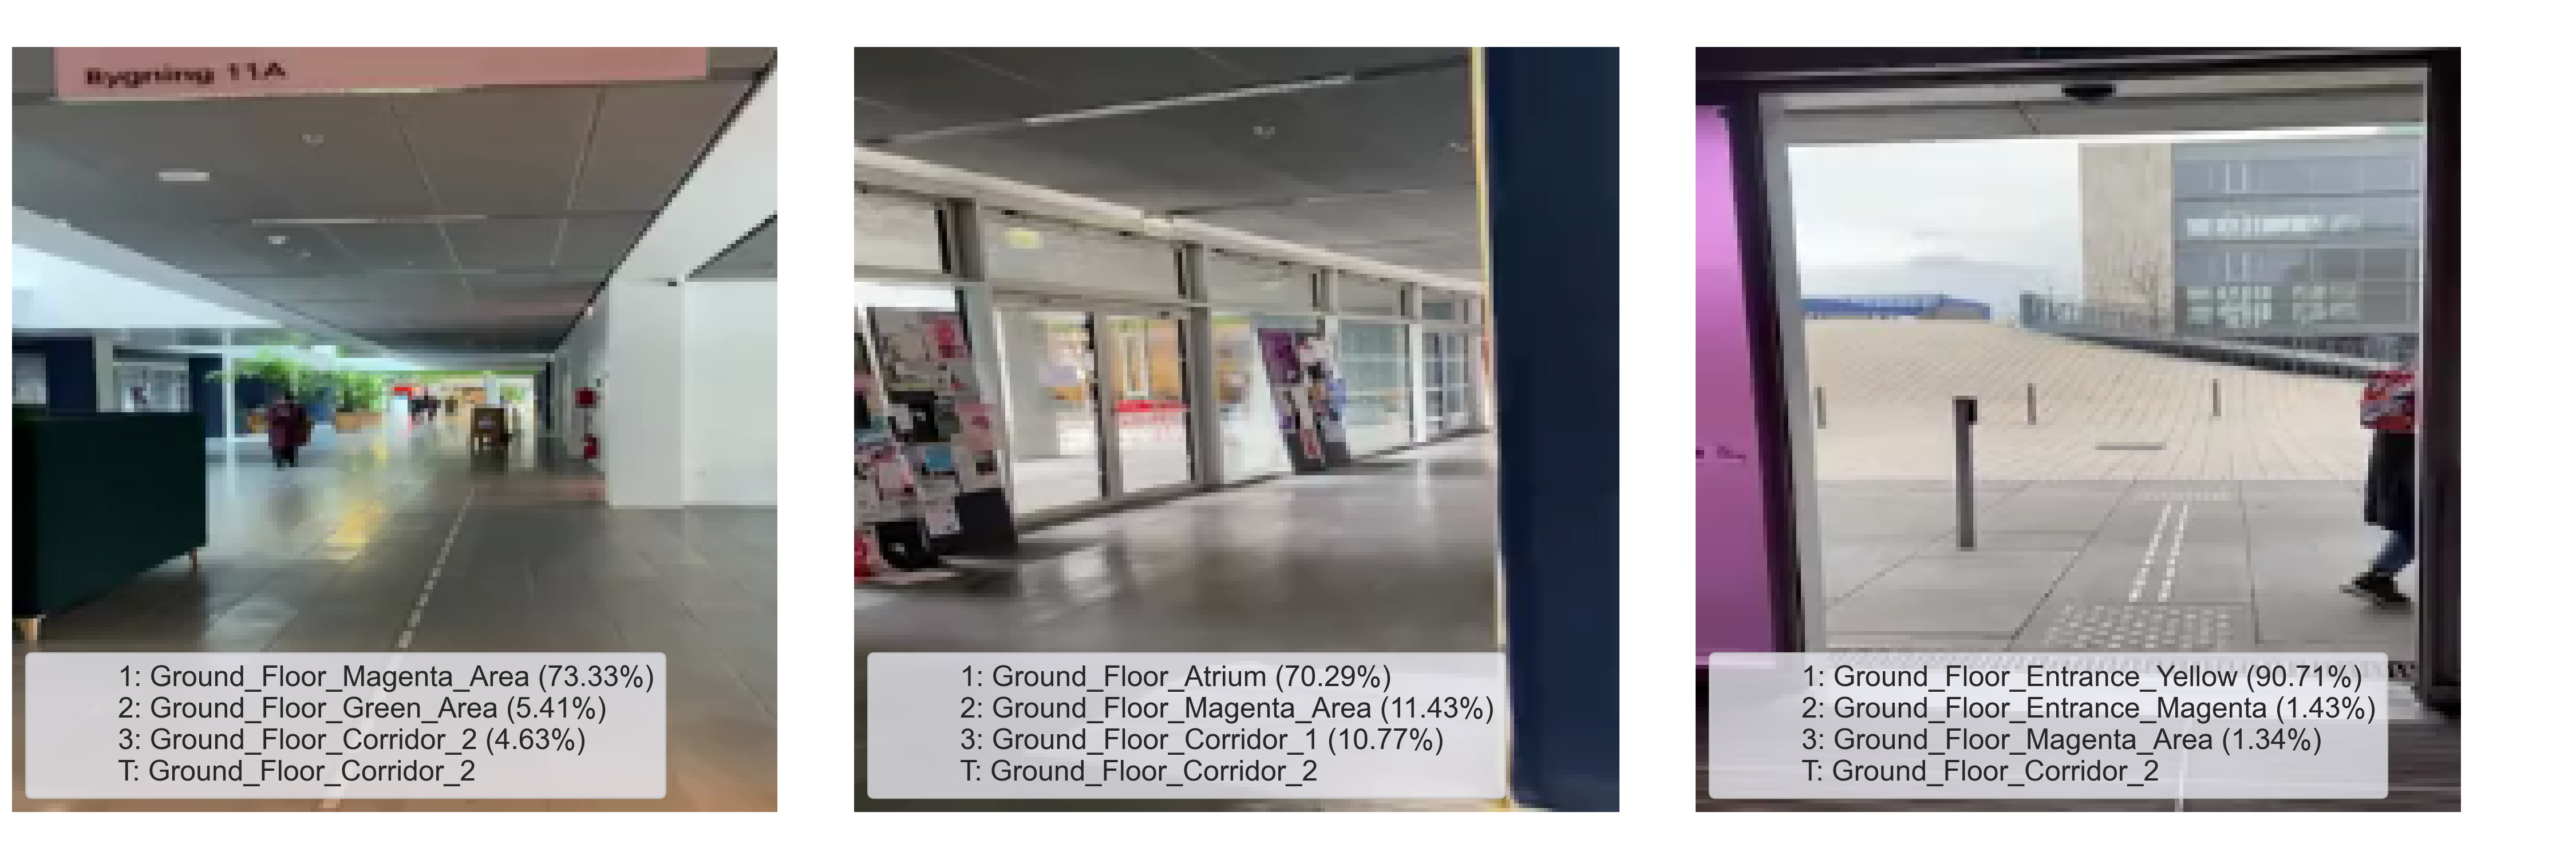
\includegraphics[width=\textwidth]{./figures/r2plus1d-mispredicted-frames.png}
\caption{R(2+1)D}
\end{subfigure}

\caption{\textbf{Mispredicted Samples.} The Figure shows the mispredicted
samples for (a) ResNet18 and (b) R(2+1)D. The respective legend shows the
top 3 predicted classes for each sample in order of confidence and the
ground truth label. For the clips from the video classifier, the first
frame of the clip is shown.}
\label{fig:mispredicted}
\end{figure}

% subsection mispredicted (end)

\subsection{Understanding Model Behaviour: Manual Inspection} % (fold)
\label{sub:manual}

Finally, the continuous predictions of the two best performing model, ResNet18
and R(2+1)D, are manually inspected on all videos in the test split. The
following qualitative observations were made:

\begin{enumerate} 

\item \textbf{Noise Invariance.} Both models show a high robustness to temporal
  changes in the environment, such as changing lighting conditions, different
  people in the scene or occlusions. This is especially true for R(2+1)D, which
  is likely due to the temporal modelling capabilities of the model. However,
  drastic changes in the environment, such as the repainting of an entire
  region, lead to consistent mispredictions of the affected area. This is a
  general drawback of localisation systems that solely rely on the modality of
  vision 

\item \textbf{Prediction Robustness.} A noticeable difference in terms of the
  sample-to-sample variance could be observed. ResNet18 was found more prone to
  "jittering" predictions, meaning that within a single second, it would predict
  different classes. Such behaviour was almost entirely absent in R(2+1)D, due
  to the lower throughput rate and its temporal modelling capabilities.

\item \textbf{Low-Resource Classes.} Both models struggle with underrepresented
  clases and features, like unusual routes or angles. The higher the deviance
  from the training data, the less certain the models are about their
  predictions, which often leads to mispredictions. Given this, performance
  gains are to be expected for large-scale, exhaustive training data collection.
  In contrast, classes that show distinctive features, such as the Atrium or
  First Floor Mezzanine, are predicted more reliably.

\item \textbf{Training Data Bias.} A bias toward the training data is present in
  both models. If features that are not representative of a class, but are
  overrepresented in the training data of that class, there is a chance for the
  model to learn these features as being indicative of a class. This was the
  case for the libraries: Most video clips that were taken while walking through
  bookshelves were filmed in library 2, while the other libraries were filmed in
  a more open space. This led to model associating in-between bookshelves clips
  to library 2, even though they are also present in the other libraries. When
  used in practice, data collection has to be carefully designed to avoid such
  biases.

\end{enumerate}

% subsection manual (end)

\subsection{Deployment on Mobile Devices}
\label{sub:deploment}

As a proof of concept, the best single-frame classifier, ResNet18, was deployed
on a mobile device. The trained model was quantised to 8-bit float precision and
converted to \texttt{TorchScript} format to be run more efficiently on mobile
devices. Deployment was done using the \texttt{PlayTorch}
framework, which is a port of the \texttt{PyTorch} Mobile SDK
for native iOS and Android to Javascript. The deployed model can be tested by
downloading the PlayTorch app from the App Store or Google Play Store and
scanning the QR code found in the \href{https://github.com/mikasenghaas}{README}
of this project's GitHub repository. This will open the application, download
the model and run it locally on the device.

% subsection deployment (end)

% section results (end)

\section{Limitations \& Future Work} % (fold)
\label{sec:discussion}

This study has shown the potential of using a pure deep learning pipeline for
tackling the problem of indoor localisation. However, there are still many
open questions that need to be addressed in future work for systems similar to
the approach suggested here to be widely useful in real-world applications.

% coarse location labels
The main drawback of the proposed approach is the coarse location labels.
State-of-the-art indoor localisation systems are able to localise users to
centimetre accuracy. Therefore, future work should focus making improvements
on the entire pipeline that allow for higher precision in the location labels.

% small data set
Furthermore, this study assumes a small data set of only 40 minutes of video
footage for training. While the experiment setup allowed to draw conclusion
about the data efficiency of the models and the general feasibility of the
data collection and annotation process, it is an open question how similar
systems scale to even larger indoor spaces with more training data available.

% representativeness of test split
Additionally, it has to be noted that the test split was collected over a
duration of four different days in close succession. Therefore, the test split
might not be representative of the true variation of visual inputs from a
indoor location over the course of a year. For example, the location might
change more significantly than represented in the test split over seasons.
In that case, the reported test metrics are likely to be over-optimistic. To
gain confidence in favour or against this hypothesis, monitoring the
performance of the trained models on test data collected over a longer period
of time would be necessary.

% edge-cases
Finally, the detailed analysis of the mispredicted samples has shown that
most errors, because the models that show a lot of similar features, such as
different libraries, or rooms that are architecturally similar across floors.
Future work should specifically improve on finding solutions to these issues.
Possible starting points might be to use the fact that sudden jumps in the
building are impossible, so highly confident predictions from the past can be
used as a strong indicator for the next room if some knowledge about the
relative position of the rooms is available.

Due to different nature of the underlying datasets $D_f$ and $D_v$, one
containing a set of frames, the other containing a set of clips,  the
performance and efficiency metrics are not directly comparable.

For example, the top-1 accuracy of the single-frame classifiers is the number of
correctly predicted frames, whereas the top-1 accuracy of the video classifiers
is the number of correctly predicted videos. While this limits the comparability
of the metrics, it is still possible to draw conclusion between the different
model types due to the relatively large number of samples and the natural
resemblance of frames and clips.

% section Discussion (end)

\section{Conclusion} % (fold)
\label{sec:conclusion}

% indoor localisation is solvable with a pure deep learning pipeline
The study has shown promising results for the feasibility of a pure deep
learning pipeline for indoor localisation.

% single-frame classifiers
Surprisingly, the single-frame classifier ResNet18 was able to achieve a test
accuracy of 70\%. This is a promising result, given that the model was trained
on less than 40 minutes of training video footage in a 20 room indoor
location. It is found that video classification models are able to improve the
overall performance of the system noticeably. However, the performance gains
come at the cost of a higher computational complexity, which only allows for
near real-time inference. 

Depending on the application, the trade-off between performance and
computational complexity can lead to one or the other architecture being
preferred.

% main drawbacks, failure modes
All models struggle with low-resource classes, visually similar classes and
biases in the training data. All of these issues are grounded in the nature of
the data set and the problem itself. Future work should focus on improving the 
data collection process by, for example, scaling it to larger indoor locations,
be mindful of biases in the training data and investigate augmentation
techniques to improve the robustness of the models.


% section conclusion (end)

% bibliography
\newpage
\bibliography{references}
\bibliographystyle{abbrv}


\newpage
\section{Appendix} % (fold)
\label{sec:appendix}

\subsection{Reproducibility} % (fold)
\label{sub:reproducibility}

All code and data used in this project is available on
\href{https://github.com/mikasenghaas/bsc}{GitHub}. The project's
\texttt{README} file contains detailed instructions on how to reproduce the
results of this project.

Further, the precise configuration and results of the experiments that are
reported here are publicly available as a public
\href{https://wandb.ai/mikasenghaas/bsc}{Weights \& Biases} experiments.

% subsection reproducibility (end)

\subsection{Machine Specifications} % (fold)
\label{sub:machine-specs}

Table~\ref{tab:machine-specs} lists the two machines, alongside relevant
specifications, that were used for training and evaluation of the models.
The HPC cluster was used for training and evaluation of all models. Analyses
and visualisations were performed on the local machine, as well as running the
real-time inference demo. 

\begin{table}
\centering

\begin{subtable}{0.9\linewidth}
\centering
\begin{tabular}{cll}

\toprule
& Specification & Value \\
\midrule

\multirow{2}{*}{\rotatebox[origin=c]{90}{Sys.}} & Name & Darwin \\
\vspace{0.1cm}
& Node & MacBook Pro \\

\multirow{4}{*}{\rotatebox[origin=c]{90}{CPU}} & Model & Apple M1 \\
& Architecture & ARM64 \\
& Physical Cores & 8 \\
\vspace{0.1cm}
& Frequency & 2.4 GHz \\

\multirow{2}{*}{\rotatebox[origin=c]{90}{Mem.}} & Total Capacity & 16
GB\\
& Avg. Used Capacity & $\sim 7.4$ GB \\

\bottomrule
\end{tabular}

\caption{Local Machine}
\end{subtable}

\bigskip

\begin{subtable}{0.9\linewidth}
\centering
\begin{tabular}{cll}

\toprule
& Specification & Value \\
\midrule

\multirow{2}{*}{\rotatebox[origin=c]{90}{Sys.}} 
& Name & Linux \\
\vspace{0.1cm}
& Node & Desktop 24 \\

\multirow{4}{*}{\rotatebox[origin=c]{90}{CPU}}
& Model & Intel(R) Xeon(R) CPU E5-2660 v3 @ 2.60GHz \\
& Architecture & x86\_64 \\
& Physical Cores & 20 \\
\vspace{0.1cm}
& Frequency & 3.3 GHz \\

\multirow{2}{*}{\rotatebox[origin=c]{90}{GPU}} 
& Model & NVIDIA GeForce GTX 1080 Ti \\
\vspace{0.1cm}
& Memory & 11.2 GB \\

\multirow{2}{*}{\rotatebox[origin=c]{90}{Mem.}}
& Total Capacity & 250  
GB\\
& Avg. Used Capacity & $\sim 7.4$ GB \\

\bottomrule
\end{tabular}

\caption{HPC (Remote Server)}
\end{subtable} 

\caption{\textbf{Machine Specifications.} The Table shows relevant hardware
  specifications for (a) the local machine and (b) the remote server that were
  used for conducting experiments within this study.}

\label{tab:machine-specs}
\end{table}

% section remarks (end)

% encoding 
% \begin{table}[ht]
%   \centering
%   \begin{tabular}{lc}
%   \toprule
%   \bfseries Class & \bfseries Encoding \\
%   \midrule
%   First\_Floor\_Corridor\_1 & A \\
%   First\_Floor\_Corridor\_2 & B \\
%   First\_Floor\_Green\_Area & C \\
%   First\_Floor\_Library\_1 & D \\
%   First\_Floor\_Library\_2 & E \\
%   First\_Floor\_Library\_3 & F \\
%   First\_Floor\_Magenta\_Area & G \\
%   First\_Floor\_Mezzanine & H \\
%   First\_Floor\_Red\_Area & I \\
%   First\_Floor\_Yellow\_Area & J \\
%   Ground\_Floor\_Atrium & K \\
%   Ground\_Floor\_Corridor\_1 & L \\
%   Ground\_Floor\_Corridor\_2 & M \\
%   Ground\_Floor\_Entrance\_Magenta & N \\
%   Ground\_Floor\_Entrance\_Yellow & O \\
%   Ground\_Floor\_Green\_Area & P \\
%   Ground\_Floor\_Magenta\_Area & Q \\
%   Ground\_Floor\_Red\_Area & R \\
%   Ground\_Floor\_Yellow\_Area & S \\
%   Stairs\_Atrium & T \\
%   \bottomrule
%   \end{tabular}
%   \caption{Encoding of Classes}
%   \label{tab:class-encoding}
% \end{table}

% section appendix (end)

\end{document}
